\documentclass[11pt,aps,preprint,nofootinbib,superscriptaddress,tightenlines]{revtex4-2}
\usepackage[T1]{fontenc}
\usepackage{amsmath,amssymb,mathtools}
\let\lambdabar\relax   % revtex defines it; newpxmath does too
\usepackage{newpxtext,newpxmath}
\usepackage{bm}
\usepackage[final]{microtype}
\usepackage{xcolor}
\usepackage{booktabs}
\usepackage{graphicx}
\usepackage{dsfont}
\usepackage[most]{tcolorbox}
\usepackage{algpseudocode}
\newcommand{\one}{\mathds{1}}
\newcommand{\avg}[1]{\langle #1\rangle}
\definecolor{darkblue}{RGB}{20,60,140}
\definecolor{accent}{RGB}{30,80,150}
\definecolor{tint}{RGB}{243,246,251}
% algorithms: a titled, tinted box
\newtcolorbox{algobox}[1]{enhanced, colback=tint, colframe=accent, boxrule=0.6pt, arc=2pt,
  left=6pt, right=6pt, top=4pt, bottom=4pt, fonttitle=\bfseries\small, coltitle=white,
  colbacktitle=accent, title={#1}, before skip=10pt, after skip=10pt}
% the central equations: a tinted panel with an accent rule on the left
\newtcolorbox{keyeq}{enhanced, colback=tint, frame hidden, borderline west={2pt}{0pt}{accent},
  sharp corners, left=4pt, right=4pt, top=0pt, bottom=0pt, before skip=6pt, after skip=6pt}
\usepackage[colorlinks=true,linkcolor=darkblue,citecolor=darkblue,urlcolor=darkblue]{hyperref}

\def\st{\begin{equation}}
\def\stp{\end{equation}}
\def\Eq#1{eq.~(\ref{#1})}
\def\Sect#1{Sect.~\ref{#1}}
\def\App#1{Appendix~\ref{#1}}
\def\Fig#1{Fig.~\ref{#1}}
\def\tr{\operatorname{tr}}
\let\oldparagraph\paragraph
\renewcommand{\paragraph}{\par\bigskip\oldparagraph}

\begin{document}

\title{The partition function of the particle model:\\ thermodynamics, renormalization and the positions}
\author{D.~Teaney}
\affiliation{Department of Physics and Astronomy, Stony Brook University,
Stony Brook, New York 11794, USA}
\date{\today}

\begin{abstract}
We compute the canonical partition function of the particle model in two stages.  With every particle at the mean volume it gives the
thermodynamics of the model: the input fluid, plus an ideal gas of labels and the fluctuations of each particle, both of relative order one over
the entropy per particle.  The labels are a conserved number that the target fluid does not have; for the conformal fluid they and the fluctuations
change only the temperature scale (the bare equation of state is taken up in \nolinkurl{renormalization_sph.tex}).  The density modes of the positions then give the structure factor, the pair correlation and the volume
fluctuations in closed form, and a correction to the thermodynamics of order one over the number of neighbours.  The theory agrees with hybrid Monte Carlo.
\end{abstract}

\maketitle
\tableofcontents

%=============================================================================
\section{Introduction}
\label{sec:intro}

The particle model carries a fluid on $N$ particles.  Each particle has a position, an entropy and a momentum; its volume is not a variable of its own
but follows from the positions of its neighbours through the kernel.  In equilibrium at a temperature $T$ everything about the model, its
thermodynamics and the statistics of its positions, follows from one object, the canonical partition function $\mathcal Z_N$.  This note computes it.

There are three reasons to want it.
\begin{enumerate}
\item \emph{The thermodynamics of the model} is not that of the fluid put in.  Each particle adds the energy and the pressure of its own fluctuations,
  and the particles themselves are an ideal gas of labels.  Both are cutoff effects, of order $T$ per particle.
\item \emph{The renormalization} (\nolinkurl{renormalization_sph.tex}): which function of the model should equal the target equation of state, and how to tune the bare (input)
  equation of state to meet it.
\item \emph{The structure of the positions}: the structure factor $S(k)$, the pair correlation $g(r)$ and the fluctuations of the particle volumes.
\end{enumerate}

\paragraph{Two expansions.}  The calculation is organized by two large numbers,
\st
s_a\gg1\qquad\text{and}\qquad \bar nh^2\gg1 ,
\stp
the entropy per particle and the number of neighbours in a kernel.  The first controls the integral over the entropy and the momentum of one particle at
fixed volume (\Sect{sec:one}); it plays the role of $1/\hbar$, and its one-loop term is the origin of every correction to the thermodynamics.  The
second controls the integral over the positions (\Sect{sec:modes}).  The two are nested: the positions see a particle only through how its weight
depends on its volume.

\paragraph{The plan.}  First every particle is given the mean volume.  This already gives the thermodynamics (\Sect{sec:uniform}) and the
renormalization (\Sect{sec:ren}).  Then the density modes of the positions are added (\Sect{sec:modes}--\ref{sec:back}), and the theory is compared with
hybrid Monte Carlo (\Sect{sec:hmc}).

\paragraph{Notation.}  The simulation is in $d=2$ with the conformal equation of state of the same dimension, $c_s^2=1/2$ (\texttt{dimension.tex}).
\begin{center}
\begin{tabular}{ll}
\toprule
symbol & meaning \\
\midrule
$T$ & temperature of the ensemble, $\partial H/\partial s$ \\
$p(T)$, $e(T)$, $s(T)$ & the input (bare) equation of state; $C_V=T\,ds/dT$ \\
$\bar n=N/L^2$, $\bar V=1/\bar n$ & mean density of particles and mean particle volume \\
$V_a=1/n_a$ & volume of particle $a$, with $n_a$ the kernel density at the particle \\
$W(r)$, $\widetilde W(k)$, $h$ & the kernel, its Fourier transform ($\widetilde W(0)=1$), its size \\
$\sigma=p(T)\bar V/T$ & the pressure of the fluid in one particle volume, over $T$ \\
$Z_1(T,V)$, $F_1=-T\ln Z_1$ & one particle at fixed volume: partition function, free energy \\
$\Pi$, $\mathcal K$ & pressure and stiffness of a particle, \Eq{PiK} \\
$\mathcal K_0=(d+1)/2$ & their one-loop value \\
$\mu$ & chemical potential of the labels \\
\bottomrule
\end{tabular}
\end{center}
For the conformal fluid
\st
p\propto T^3,\qquad e=2p,\qquad Ts=3p,\qquad C_V=2s,\qquad \sigma=\frac{s(T)\bar V}3 .
\stp

%=============================================================================
\section{The partition function}
\label{sec:Z}

\paragraph{The model.}  The energy is a sum over particles,
\st
H=\sum_ae_a(s_a,\bm m_a,V_a),\qquad V_a=\frac1{n_a},\qquad n_a=\sum_bW(\bm x_a-\bm x_b),
\stp
the sum including $b=a$.  The energy of a particle is its volume times the energy density of the input fluid, a function of the entropy density
$s_a/V_a$, the (density-frame) momentum density $\bm m_a/V_a$ and, in general, the density of particles $1/V_a$:
\st
e_a(s_a,\bm m_a,V_a)=V_a\,\varepsilon\Big(\frac{s_a}{V_a},\frac{\bm m_a}{V_a};\frac1{V_a}\Big).
\stp
The input in the code is a fluid without a charge: $\varepsilon$ does not depend on the density of particles, and the energy is extensive.  The dependence is kept
because a bare equation of state may need it (\nolinkurl{renormalization_sph.tex}).

\paragraph{The ensemble.}  In the canonical ensemble with the Liouville measure, flat in the positions, the entropies and the momenta, a configuration
has the weight
\st
\prod_a\exp\Big[s_a-\frac{e_a}{T}\Big]\;\prod_ad^2\bm x_a\,ds_a\,d^2\bm m_a .
\stp
The factor $e^{s_a}$ counts the microscopic states that a particle with entropy $s_a$ stands for; $s_a-e_a/T$ is the Massieu function of the particle.

\paragraph{The partition function.}  At fixed positions the particles are independent, because the positions enter only through the volumes.
Integrating the entropy and the momentum of each particle,
\begin{keyeq}
\st
\mathcal Z_N=\frac1{N!}\int\prod_ad^2\bm x_a\;\prod_aZ_1(T,V_a),\qquad
Z_1(T,V)=\int ds\,d^2\bm m\;\exp\Big[s-\frac{e(s,\bm m,V)}{T}\Big] .
\label{ZN}
\stp
\end{keyeq}
$Z_1$ is \emph{one} function, the same for every particle: the partition function of a single particle held at the volume $V$.  In the ensemble its
argument is the fluctuating volume $V_a$, which the positions determine.  The $N!$ is a convention; nothing at fixed $N$ depends on it.

\paragraph{Only derivatives matter.}  Scaling the measure of each particle by a constant $\lambda$ multiplies $\mathcal Z_N$ by $\lambda^N$.  This changes no
average at fixed $N$: averages are derivatives of $\ln\mathcal Z_N$ with respect to $T$, $L$ or a source, and $N\ln\lambda$ depends on none of them.  So
only the derivatives of $\ln Z_1$ with respect to $V$ and $T$ are physical; its absolute value is not.

%=============================================================================
\section{One particle at fixed volume}
\label{sec:one}

The point: the positions see a particle only through how $\ln Z_1$ depends on $V$, and the thermodynamics only through how it depends on $V$ and $T$.
At large $s_a$ the integral \Eq{ZN} is done by its saddle point.

\subsection{Tree level: the maximum}
\label{sec:tree}

Change variables to the densities, $S=s/V$ and $\bm M=\bm m/V$, and write $n=1/V$ for the density of particles:
\st
ds\,d^d\bm m=V^{d+1}\,dS\,d^d\bm M,\qquad s-\frac eT=V\,\psi(S,\bm M),\qquad \psi=S-\frac{\varepsilon(S,\bm M;n)}T ,
\stp
with $\psi$ the Massieu density.  Its maximum is at $\partial\varepsilon/\partial S=T$ and $\bm M=0$, the fluid at rest at the temperature $T$.  There it is
minus the free-energy density of the input over the temperature,
\st
\psi_{\max}=-\frac{f(T,n)}T,\qquad f=\varepsilon-TS ,
\stp
so that at tree level a particle is a piece of the input fluid of volume $V$:
\begin{keyeq}
\st
F_1\big|_{\rm tree}=V\,f\Big(T,\frac1V\Big) .
\label{Ftree}
\stp
\end{keyeq}
The input is a fluid with a charge, the density of particles $n$, with the pressure, the chemical potential and the bulk modulus
\st
p=n\frac{\partial f}{\partial n}-f,\qquad \mu_1=\frac{\partial f}{\partial n},\qquad B=n\frac{\partial p}{\partial n}\qquad\text{at fixed }T .
\stp

\paragraph{The input without a charge.}  For the fluid in the code $f$ does not depend on $n$, so
\st
f=-p(T),\qquad \mu_1=0,\qquad B=0,\qquad \ln Z_1\big|_{\rm tree}=\frac{p(T)\,V}T .
\stp
This is the one-particle form of Israel's thermodynamic potential, $\Phi^\mu=s^\mu+\beta_\nu T^{\mu\nu}=p\beta^\mu$, whose time component is $p/T$: the weight
is extensive, and the particle has a pressure but no stiffness and no chemical potential.  Below, formulas with $p(T)$ alone are for this case.

\subsection{One loop: the Gaussian integral}
\label{sec:oneloop}

At the maximum the second derivatives are
\st
\frac{\partial^2\psi}{\partial S^2}=-\frac1{C_V},\qquad \frac{\partial^2\psi}{\partial M_i\partial M_j}=-\frac{\delta_{ij}}{T(e+p)} .
\stp
The exponent is $V\psi$, so each of the $d+1$ variables has a Gaussian width proportional to $V^{-1/2}$.  The integral is
\begin{keyeq}
\st
\ln Z_1(T,V)=\underbrace{-\frac{V f}T}_{\text{tree}}+\underbrace{\tfrac12\ln\det\big(2\pi V\chi\big)}_{\text{one loop}}+O\Big(\frac1{s_a}\Big),
\qquad \chi={\rm diag}\big(C_V,\ T(e+p)\,\delta_{ij}\big) .
\label{lnZ1}
\stp
\end{keyeq}
$\chi$ is the matrix of susceptibilities of the conserved densities carried by a particle, its entropy and its $d$ momentum components.  At fixed
volume they fluctuate with
\st
\avg{\delta s_a^2}=C_V\,V,\qquad \avg{m_{a,i}\,m_{a,j}}=\delta_{ij}\,T(e+p)\,V .
\label{intrinsic}
\stp
The one-loop term is the Einstein fluctuation entropy of these $d+1$ densities.  It is not extensive: for the input without a charge, $\chi$ does not
depend on $V$, and at fixed $T$
\st
\tfrac12\ln\det\big(2\pi V\chi\big)=\mathcal K_0\ln V+\tfrac12\ln\det(2\pi\chi),\qquad \mathcal K_0=\frac{d+1}2=\frac32 .
\stp
$\mathcal K_0$ is half the number of conserved densities per particle: a larger volume gives each of them more room.

\paragraph{The size of the loop.}  $V\psi_{\max}$ is of order $s_a$, so the relative fluctuations are of order $s_a^{-1/2}$, and each further order of the
expansion about the maximum is smaller by $1/s_a$ (\App{app:single}).

\subsection{The thermodynamics of a particle}
\label{sec:particlethermo}

The free energy of a particle at fixed volume and its derivatives are
\st
F_1(T,V)=-T\ln Z_1,\qquad p_1=-\frac{\partial F_1}{\partial V}\Big|_T,\qquad B_1=-V\frac{\partial p_1}{\partial V}\Big|_T,
\stp
the pressure and the bulk modulus of a particle.  With the Liouville measure the volume enters $Z_1$ only through $e_a$, so $p_1$ is the canonical average
at fixed volume of the mechanical pressure that drives the particle,
\st
p_1=\avg{p_a}_V,\qquad p_a=-\frac{\partial e_a}{\partial V}\Big|_{s_a,\bm m_a} .
\stp
The positions need their dimensionless forms, at the mean volume:
\begin{keyeq}
\st
\Pi\equiv\frac{p_1V}T=V\frac{\partial\ln Z_1}{\partial V},\qquad
\mathcal K\equiv\frac{VB_1}T=-V^2\frac{\partial^2\ln Z_1}{\partial V^2}\qquad\text{at }V=\bar V .
\label{PiK}
\stp
\end{keyeq}
At tree level, by \Eq{Ftree}, they are the pressure and the bulk modulus of the input, $\Pi=pV/T$ and $\mathcal K=VB/T$.  The one-loop term adds
$\mathcal K_0$ to both (and, for an input with a charge, the dependence of $\chi$ on $n$).  For the input without a charge
\st
\Pi=\sigma+\mathcal K_0,\qquad \mathcal K=\mathcal K_0 .
\label{PiKloop}
\stp
A piece of a neutral fluid has a pressure but no stiffness, since its weight is linear in $V$.  The one loop adds to both, like an ideal gas of $\mathcal K_0$
particles: a particle resists compression because compressing it squeezes its own fluctuations.

\paragraph{The energy of a particle.}  The mean energy at fixed volume is
\st
\avg{e_a}_V=T^2\frac{\partial\ln Z_1}{\partial T}=V\,e(T)+\Delta e,\qquad
\Delta e=\frac T2\Big[\frac{d\ln C_V}{d\ln T}+d\,\frac{d\ln T(e+p)}{d\ln T}\Big] .
\label{Deltae}
\stp
The widths \Eq{intrinsic} grow with the temperature, so heating a particle also puts energy into its fluctuations.  For the conformal fluid
$C_V\propto T^2$ and $T(e+p)\propto T^4$, and
\st
\Delta e=5\,T .
\stp

\subsection{Small entropy per particle}
\label{sec:quadrature}

At small $s_a$ the saddle point is not enough: the light cone cuts off the momentum, and the distribution of a particle is far from Gaussian.  Then
$\ln Z_1$ is computed by quadrature (\texttt{examples/single\_particle.jl}), and $\Pi$ and $\mathcal K$ by finite differences in $V$.  At the three
temperatures of the hybrid Monte Carlo runs (\Sect{sec:hmc}):
\begin{center}
\begin{tabular}{cccccccc}
\toprule
$\sigma$ & $s(T)\bar V$ & $\Pi$ & $\Pi-\sigma$ & $\mathcal K$ & $r_s$ & $r_m$ & $\avg{s_a}/s(T)\bar V$ \\
\midrule
3.89 & 11.7 & 5.25 & 1.35 & 1.225 & 0.918 & 1.568 & 1.26 \\
16.4 & 49.2 & 17.87 & 1.46 & 1.425 & 0.969 & 1.140 & 1.07 \\
179 & 536 & 180.3 & 1.50 & 1.493 & 0.997 & 1.013 & 1.01 \\
\bottomrule
\end{tabular}
\end{center}
Here $r_s$ and $r_m$ are the entropy and momentum variances over their one-loop values \Eq{intrinsic}.  Both $\Pi-\sigma$ and $\mathcal K$ approach
$\mathcal K_0=3/2$ at large $\sigma$.  At $\sigma=3.89$ the momentum variance is $57\%$ above the Gaussian, and the particle has fewer effective
phase-space dimensions, $\mathcal K=1.225$.  Everything below holds with the exact $\Pi$ and $\mathcal K$ in place of \Eq{PiKloop}.

%=============================================================================
\section{The model at uniform density}
\label{sec:uniform}

The point: with every particle at the mean volume, $\mathcal Z_N$ is the input fluid, plus an ideal gas of labels, plus the fluctuations of each
particle.  This stage is exact in the particle variables and neglects only the density modes of the positions, of relative order $1/(\bar nh^2)$.

\subsection{The ideal gas of labels}
\label{sec:labelgas}

Put $V_a=\bar V$ in \Eq{ZN}.  The positions give $L^{2N}/N!$, and with Stirling's formula
\begin{keyeq}
\st
\frac{\ln\mathcal Z_N}N=\underbrace{\ln\bar V+1}_{\text{labels}}+\underbrace{\ln Z_1(T,\bar V)}_{\text{one particle}} .
\label{lnZuniform}
\stp
\end{keyeq}
The first term is the entropy of placing $N$ labelled points in the box, the second the weight of one particle.  \Sect{sec:posloop} adds the
correction from the density modes.

\subsection{Pressure and energy}
\label{sec:pe}

The pressure is the derivative with respect to the area at fixed $N$ and $T$, and the energy density the derivative with respect to $T$:
\st
p_{\rm model}=\frac{T}{N}\frac{\partial\ln\mathcal Z_N}{\partial\bar V}\Big|_{T,N},\qquad E=\frac{T^2}{L^2}\frac{\partial\ln\mathcal Z_N}{\partial T}\Big|_{\bar V,N} .
\stp
From \Eq{lnZuniform}, the pressure of the model is that of the ideal gas of labels plus that of one particle, and the energy is that of the particles:
\begin{keyeq}
\st
p_{\rm model}=\bar nT+p_1(T,\bar V),\qquad E=\bar n\,\avg{e_a}_{\bar V} .
\label{pE}
\stp
\end{keyeq}
This holds for any input.  For the input without a charge, at one loop (\Eq{PiKloop} and \Eq{Deltae}),
\st
p_{\rm model}=p(T)+(1+\mathcal K_0)\,\bar nT,\qquad E=e(T)+\bar n\,\Delta e .
\label{pEloop}
\stp
The model has the pressure and energy of the input fluid plus terms of order $T$ per particle:

\begin{itemize}
\item \emph{$\bar nT$, the label pressure}, from the entropy of placing the points.  It is the kinetic stress of the particles' thermal motion: with the velocity
  $\bm v_a=\partial e_a/\partial\bm m_a$, equipartition holds for any shape of the energy,
  \st
  \avg{\bm m_a\cdot\bm v_a}=d\,T,\qquad \frac1{dL^2}\Big\langle\sum_a\bm m_a\cdot\bm v_a\Big\rangle=\bar nT ,
  \stp
  and the momentum flux of the model contains $\sum_a\bm m_a\bm v_a$.  It is measured as $\tau^{\rm kin}$ (\texttt{statics.tex}).
\item \emph{$\mathcal K_0\bar nT$ and $\bar n\Delta e$}, the pressure and the energy of each particle's own fluctuations, the one-loop term of \Eq{lnZ1}.
\end{itemize}

Relative to the fluid both are of order $1/\sigma$.  For the conformal fluid
\st
\frac{(1+\mathcal K_0)\bar nT}{p}=\frac{2.5}\sigma,\qquad \frac{\bar n\Delta e}{e}=\frac{2.5}\sigma ,
\stp
which is $64\%$, $15\%$ and $1.4\%$ at the $\sigma=3.89$, $16.4$, $179$ of the runs.  These are the cutoff terms of fluctuating hydrodynamics, of
order $T\Lambda^d$ with the density of particles as the cutoff, $\Lambda^d\sim\bar n$.

\subsection{The labels as a conserved charge}
\label{sec:charge}

The fluid put in has no conserved particle number, but the model does: $N$ is fixed.  So the model is a fluid with a charge, the labels, and a chemical
potential
\st
-\frac\mu T=\frac{\partial\ln\mathcal Z_N}{\partial N}\Big|_{T,L}=\ln\bar V+\ln Z_1(T,\bar V)-\Pi .
\label{mu}
\stp
At one loop the fluid term $pV/T$ cancels between $\ln Z_1$ and $\Pi$, and
\st
-\frac\mu T=(1+\mathcal K_0)\ln\bar V+\tfrac12\ln\det\big(2\pi\chi(T)\big)-\mathcal K_0 .
\label{muloop}
\stp
The thermodynamics of the model obeys the Euler and Gibbs--Duhem relations of a fluid with one charge,
\st
E+p_{\rm model}=Ts_{\rm model}+\mu\bar n,\qquad dp_{\rm model}=s_{\rm model}\,dT+\bar n\,d\mu ,
\label{GD}
\stp
with $s_{\rm model}$ the entropy density of the model.  The value of $\mu$ depends on the normalization of the measure, $\mu/T\to\mu/T-\ln\lambda$
(\Sect{sec:Z}); its derivatives do not.  For the conformal fluid the temperature drops out of \Eq{muloop}:
\st
-\frac\mu T=(1+\mathcal K_0)\ln\big(s(T)\bar V\big)+\text{const} .
\label{muconf}
\stp

\paragraph{Two pressures.}  The ``Euler'' pressure $T\ln\mathcal Z_N/L^2$ and the mechanical pressure $p_{\rm model}$ differ by $\bar n\mu$.  The first moves with
the normalization; the second is the measured stress and does not.  Below, the pressure is always the mechanical one.

\subsection{The compressibility of the labels}
\label{sec:S0}

At fixed temperature the pressure of the model depends on the density of particles.  Differentiating \Eq{pE}, the label gas gives $T$ and the particle its bulk modulus, $\partial p_1/\partial\bar n=\bar VB_1=T\mathcal K$ by \Eq{PiK}:
\st
\frac{\partial p_{\rm model}}{\partial\bar n}\Big|_T=T\,(1+\mathcal K) .
\stp
By the compressibility sum rule the long-wavelength fluctuations of the number of particles are
\begin{keyeq}
\st
S(0)=T\frac{\partial\bar n}{\partial p_{\rm model}}\Big|_T=\frac{1}{1+\mathcal K}\;\simeq\;\frac{1}{1+\mathcal K_0}=\frac25 .
\label{S0}
\stp
\end{keyeq}
Poisson, $S(0)=1$, would be an ideal gas of points.  The particles are stiffer by $1+\mathcal K$: the $1$ from placing the points, the $\mathcal K$ from the
stiffness of each particle.  The fluid's pressure drops out, because at long wavelength moving particles relabels the fluid without changing it.
\Sect{sec:S0check} recovers \Eq{S0} from the density modes.

\subsection{Connection with hydro-kinetic theory}
\label{sec:amt}

In hydro-kinetic theory \cite{amt} the fluctuations of the $n_\Lambda$ hydrodynamic modes per unit volume below the cutoff renormalize a bare equation of
state $e_0$, $p_0$ (eq.~(35) there, written for $d$ dimensions):
\st
e=e_0+d\,Tn_\Lambda,\qquad p=p_0+\Big[1+\frac T2\frac{dc_s^2}{dT}\Big]Tn_\Lambda .
\label{amt35}
\stp
The three terms are the kinetic energy of the momentum fluctuations, $\avg{\bm M^2}/(e+p)$; their kinetic stress; and the curvature of the equation of state
acting on the energy fluctuations, $\tfrac12p''(e)\avg{\delta e^2}$.  One particle is one mode, $n_\Lambda\leftrightarrow\bar n$, and the model has the same three
terms (\nolinkurl{renormalization_sph.tex}, Appendix), with the bare function the mean rest-frame energy density of a particle, $\bar e_{\rm rest}=\avg{e_{{\rm rest},a}}$:
\st
E=\bar e_{\rm rest}+d\,\bar nT,\qquad p_{\rm model}=p(\bar e_{\rm rest})+\Big[1+\frac T2\frac{dc_s^2}{dT}\Big]\bar nT .
\label{amtmodel}
\stp
The kinetic stress is the label pressure.  \Eq{amtmodel} contains no $\mathcal K_0$.  It enters only through the mean rest energy at the temperature $T$,
shifted from the input by the skewness of the particle's distribution,
\st
\bar e_{\rm rest}(T)=e(T)+\bar n\,\frac T{c_s^2}\Big[\mathcal K_0-\frac T2\frac{dc_s^2}{dT}\Big] ,
\stp
which turns \Eq{amtmodel} into \Eq{pEloop}.  Eliminating $\bar e_{\rm rest}$ instead, the measured pressure as a function of the measured energy is
\begin{keyeq}
\st
p_{\rm model}=p(E)+\Big[1-d\,c_s^2+\frac T2\frac{dc_s^2}{dT}\Big]\bar nT .
\label{PofE}
\stp
\end{keyeq}
For the conformal fluid, $d\,c_s^2=1$, the bracket vanishes: the model's $p(E)$ is the input one.  At one loop the labels and the fluctuations change the
temperature scale, not the equation of state.

%=============================================================================
\section{Renormalization}
\label{sec:ren}

The model's thermodynamics differs from the input at order $1/\sigma$, so the input is a bare equation of state, and the labels give the model a second
variable.  What the bare equation of state should be is taken up in \nolinkurl{renormalization_sph.tex}.  In brief: the mechanics uses the pressure as a function of the
energy density, \Eq{PofE}, which for the conformal fluid is the input one at one loop, at every density of particles.  The labels and the fluctuations change
only the temperature scale.  Along a curve of fixed $\mu/T$, on which the density of particles follows the entropy,
\begin{keyeq}
\st
P(T)=p(T)\Big[1+\frac{1+\mathcal K_0}\sigma\Big],\qquad E(T)=e(T)+5\,\bar nT=2P(T) ,
\label{Pconf}
\stp
\end{keyeq}
a change of the Stefan--Boltzmann constant, which is seen where the temperature enters explicitly, in the transport coefficients.

\section{The positions: density modes}
\label{sec:modes}

The point: the volumes are not all equal; they fluctuate with the positions.  To second order in the density of points the weight of the positions is
Gaussian, and this gives the structure factor in closed form, with the two numbers $\Pi$ and $\mathcal K$ of \Eq{PiK} as its only input.

\subsection{The weight as a functional of the density}
\label{sec:functional}

Define the density of points and the kernel density,
\st
\rho(\bm x)=\sum_a\delta(\bm x-\bm x_a),\qquad n(\bm x)=(W*\rho)(\bm x),
\stp
so that $n_a=n(\bm x_a)$.  A sum over particles is an integral against $\rho$, and the weight of the positions in \Eq{ZN} is
\st
\sum_a\ln Z_1(V_a)=\int d^2x\;\rho(\bm x)\,\ln Z_1\Big(\frac1{n(\bm x)}\Big) .
\stp
Fourier components in the box are $\rho_{\bm k}=\sum_ae^{-i\bm k\cdot\bm x_a}$, and $n_{\bm k}=\widetilde W(k)\rho_{\bm k}$.  For the Wendland kernels
$0\le\widetilde W\le1$ (\App{app:kernels}).

\subsection{Second order}
\label{sec:second}

Write $\delta_a=\delta n(\bm x_a)/\bar n$.  In the variable $\ln V$ the derivatives of $\ln Z_1$ are $\Pi$ and $\Pi-\mathcal K$, and with
$\delta\ln V_a=-\delta_a+\tfrac12\delta_a^2$,
\st
\sum_a\ln Z_1(V_a)=N\ln Z_1(\bar V)-\Pi\sum_a\delta_a+\Big(\Pi-\frac{\mathcal K}2\Big)\sum_a\delta_a^2+\dots
\stp
Both sums are quadratic in the density modes (the first because the density seen from a particle is correlated with the particle being there):
\st
\sum_a\delta_a=\frac1{\bar nL^2}\sum_{\bm k}\widetilde W\,|\delta\rho_{\bm k}|^2,\qquad
\sum_a\delta_a^2=\frac1{\bar nL^2}\sum_{\bm k}\widetilde W^2\,|\delta\rho_{\bm k}|^2 .
\stp
So the weight of the positions is
\begin{keyeq}
\st
\sum_a\ln Z_1(V_a)=N\ln Z_1(\bar V)-\frac1{2\bar nL^2}\sum_{\bm k}A(k)\,|\delta\rho_{\bm k}|^2,\qquad
A(k)=2\Pi\,\widetilde W\big(1-\widetilde W\big)+\mathcal K\,\widetilde W^2 .
\label{Ak}
\stp
\end{keyeq}

\paragraph{What the two terms penalize.}  The $\Pi$ term, mostly the total volume of the particles, vanishes at both ends.  At $kh\to0$ the kernel
resolves the density, $n=\rho$, and the total volume $\int\rho/n$ is the area of the box: moving particles at long wavelength relabels the fluid without
changing it.  At $kh\to\infty$ the kernel averages the fluctuation away.  Only fluctuations on the scale of the kernel cost the fluid's pressure.  The
$\mathcal K$ term is the stiffness of the particles, which survives at $k\to0$.

\subsection{The partition function as an integral over the density}
\label{sec:Sk}
\label{sec:posloop}

The point: to second order the positions enter the weight only through the density modes $\delta\rho_{\bm k}$, \Eq{Ak}, so the integral over the $N$ positions can
be traded for an integral over the modes.  It is then Gaussian, and gives both the structure factor and the partition function.

\paragraph{From positions to density modes.}  Any function of the positions that depends on them only through the density, $F[\rho]$, can be integrated
over the modes instead,
\st
\int\frac{\prod_ad^2\bm x_a}{N!}\,F[\rho]=\int\mathcal D\rho\;\Omega[\rho]\,F[\rho],\qquad
\mathcal D\rho=\prod_{\bm k\neq0}{}^{'}\,d^2\rho_{\bm k} ,
\stp
with one complex variable per pair $\pm\bm k$ (since $\rho_{-\bm k}=\rho_{\bm k}^*$; the mode $\bm k=0$ is fixed by $N$).  $\Omega[\rho]$ counts the
arrangements of the $N$ points that have the given modes, and $\ln\Omega$ is the entropy of the arrangement.  For points placed independently and
uniformly each mode $\rho_{\bm k}=\sum_ae^{-i\bm k\cdot\bm x_a}$ is a sum of $N$ unit phases, by the central limit theorem a complex Gaussian with
$\avg{|\delta\rho_{\bm k}|^2}=N$, so
\st
\ln\Omega[\rho]=-\frac1{2N}\sum_{\bm k\neq0}|\delta\rho_{\bm k}|^2+\text{const},\qquad
\int\mathcal D\rho\;\Omega[\rho]=\frac{L^{2N}}{N!} ,
\stp
the constant fixed by the second relation, the ideal gas of labels.  The sum runs over all $\bm k\neq0$, so each pair appears twice.

\paragraph{The Massieu functional of the density.}  With $F=\prod_aZ_1(V_a)$ and \Eq{Ak}, $N=\bar nL^2$,
\begin{keyeq}
\st
\begin{aligned}
\mathcal Z_N&\simeq\int\mathcal D\rho\;e^{\Phi[\rho]},\qquad
\Phi[\rho]=\underbrace{\ln\Omega[\rho]}_{\text{arrangement}}+\underbrace{\sum_a\ln Z_1(V_a)}_{\text{particles}},\\
\Phi[\rho]&=N\ln Z_1(\bar V)-\frac1{2N}\sum_{\bm k\neq0}\big[1+A(k)\big]\,|\delta\rho_{\bm k}|^2+\text{const}.
\end{aligned}
\label{action}
\stp
\end{keyeq}
$\Phi$ is the logarithm of the weight of a density profile, as $s-e/T$ is that of a particle.  The $1$ is the entropy of the arrangement, which alone
would make the points an ideal gas; $A(k)$ is the weight of the particles, which correlates them.

\paragraph{The structure factor.}  Each pair $\pm\bm k$ is a complex Gaussian with the weight $\exp[-(1+A)|\delta\rho_{\bm k}|^2/N]$, so
\begin{keyeq}
\st
S(k)=\frac{\avg{|\delta\rho_{\bm k}|^2}}N=\frac1{1+A(k)}=\frac{1}{1+2\Pi\,\widetilde W(1-\widetilde W)+\mathcal K\,\widetilde W^2} .
\label{Sk}
\stp
\end{keyeq}
The pair correlation is its Fourier transform,
\st
\bar n\,\big[g(r)-1\big]=\int\frac{d^2k}{(2\pi)^2}\,e^{i\bm k\cdot\bm r}\,\big[S(k)-1\big] .
\stp

\paragraph{The partition function.}  Relative to the ideal gas each pair contributes the ratio of Gaussian integrals
\st
\frac{\int d^2z\;e^{-(1+A)|z|^2/N}}{\int d^2z\;e^{-|z|^2/N}}=\frac1{1+A(k)}=S(k),
\stp
so, with $\sum_{\bm k}\to L^2\int d^2k/(2\pi)^2$ and each pair counted once, \Eq{lnZuniform} becomes
\begin{keyeq}
\st
\frac{\ln\mathcal Z_N}N=\underbrace{\ln\bar V+1}_{\text{labels}}+\underbrace{\ln Z_1(T,\bar V)}_{\text{one particle}}
+\underbrace{\frac1{2\bar n}\int\frac{d^2k}{(2\pi)^2}\,\ln S(k)}_{\text{positions, one loop}} .
\label{lnZN}
\stp
\end{keyeq}
The last term is the determinant of the density modes, whose propagator is $S(k)$.  It converges, since $S\to1$ at large $k$, and it is negative:
correlating the positions lowers the entropy below that of independent particles at the mean volume.  Per particle it is of order $1/(\bar nh^2)$.

\subsection{The structure factor as a response}
\label{sec:response}

The point: $S(k)$ is the response of $\ln\mathcal Z_N$ to a potential acting on the labels.  Turning the question around, the cost of holding the labels at
a given density, shows what $A(k)$ is: the curvature of the particles' weight as a functional of the density.

\paragraph{A one-body source.}  Add a potential $U(\bm x)$ acting on the particles, and write $J=-U/T$:
\st
\mathcal Z_N[J]=\frac1{N!}\int\prod_ad^2\bm x_a\,\prod_aZ_1(V_a)\,\exp\Big[\int d^2x\,J(\bm x)\,\rho(\bm x)\Big] .
\stp
Each derivative brings down a density, so $\ln\mathcal Z_N[J]$ generates the mean density and its connected correlator:
\begin{keyeq}
\st
\frac{\delta\ln\mathcal Z_N}{\delta J(\bm x)}=\avg{\rho(\bm x)}_J\equiv\bar\rho(\bm x),\qquad
\frac{\delta^2\ln\mathcal Z_N}{\delta J(\bm x)\,\delta J(\bm y)}=\avg{\delta\rho(\bm x)\,\delta\rho(\bm y)}_J\equiv G(\bm x,\bm y) .
\label{Ssource}
\stp
\end{keyeq}
At $J=0$ the correlator depends on $\bm x-\bm y$ only, and its Fourier transform is $\bar n\,S(k)$.  This is exact.

\paragraph{The cost of a density profile.}  $\ln\mathcal Z_N[J]$ answers the question: given a potential, what density does it produce?  The labels pose the
converse: what does it cost to hold the density at a profile $\bar\rho(\bm x)$?  The Legendre transform answers it, in four steps.
\begin{enumerate}
\item \emph{Define} the effective action of the mean density,
  \st
  \Gamma[\bar\rho]=\int d^2x\,J\,\bar\rho-\ln\mathcal Z_N[J],
  \stp
  with $J$ the potential that produces $\bar\rho$.  $-\Gamma[\bar\rho]$ is the logarithm of the weight of the profile.
\item \emph{Its first derivative is the potential} needed to hold the profile, and its second derivative is therefore the inverse of the correlator:
  \st
  \frac{\delta\Gamma}{\delta\bar\rho(\bm x)}=J(\bm x),\qquad
  \frac{\delta^2\Gamma}{\delta\bar\rho\,\delta\bar\rho}=\frac{\delta J}{\delta\bar\rho}=G^{-1},\qquad
  \frac{\delta^2\Gamma}{\delta\bar\rho\,\delta\bar\rho}\bigg|_{\bm k}=\frac1{\bar n\,S(k)} .
  \label{Gamma2}
  \stp
  The curvature of $\Gamma$ is the inverse structure factor: a stiff profile fluctuates little.
\item \emph{Evaluate $\Gamma$} to the order of the Gaussian theory.  It has two pieces, the entropy of placing the labels with the mean density $\bar\rho$, and the
  weight of the particles whose volumes are set by the smoothed mean density:
  \st
  \Gamma[\bar\rho]\simeq\underbrace{\int d^2x\,\bar\rho\,\big(\ln\bar\rho-1\big)}_{\text{ideal gas of labels}}
  \;-\;\underbrace{\ln Z_{\rm part}[\bar\rho]}_{\text{weight of the particles}},
  \stp
  with
  \st
  \ln Z_{\rm part}[\bar\rho]\equiv\int d^2x\,\bar\rho\,\ln Z_1\Big(\frac1{W*\bar\rho}\Big) .
  \stp
\item \emph{Differentiate twice} at the uniform density.  The ideal gas gives $1/\bar n$.  For the particles write $\ln Z_1$ as a function of the density,
  whose first two derivatives at $\bar n$ follow from \Eq{PiK},
  \st
  \frac{\partial\ln Z_1}{\partial n}=-\frac{\Pi}{\bar n},\qquad \frac{\partial^2\ln Z_1}{\partial n^2}=\frac{2\Pi-\mathcal K}{\bar n^2} .
  \stp
  The density appears once outside the logarithm and once inside through $W*\bar\rho$, so in Fourier components
  \st
  \begin{aligned}
  \frac{\delta^2\ln Z_{\rm part}}{\delta\bar\rho\,\delta\bar\rho}\bigg|_{\bm k}&=2\widetilde W\,\frac{\partial\ln Z_1}{\partial n}+\bar n\,\widetilde W^2\,\frac{\partial^2\ln Z_1}{\partial n^2}\\
  &=-\frac1{\bar n}\Big[2\Pi\,\widetilde W\big(1-\widetilde W\big)+\mathcal K\,\widetilde W^2\Big]=-\frac{A(k)}{\bar n} .
  \end{aligned}
  \stp
\end{enumerate}
Together, with \Eq{Gamma2},
\begin{keyeq}
\st
\frac{\delta^2\Gamma}{\delta\bar\rho\,\delta\bar\rho}\bigg|_{\bm k}=\frac{1+A(k)}{\bar n}\qquad\Longrightarrow\qquad S(k)=\frac1{1+A(k)} .
\stp
\end{keyeq}
This is \Eq{Sk} again, now with a meaning for each term: the $1$ is the stiffness of the ideal gas of labels, and $A$ is the curvature of the particles'
weight, the interaction between the labels that the volumes induce.  At $k\to0$ the curvature is $(1+\mathcal K)/\bar n=\partial(\mu/T)/\partial\bar n$, the
compressibility sum rule of \Sect{sec:S0}.  (In the theory of liquids $-A/\bar n$ is the direct correlation function, and $S=1/(1+A)$ the Ornstein--Zernike
relation.)  Corrections to $\Gamma$ from the loops of the positions correct $A$, order by order in $1/(\bar nh^2)$.

\paragraph{Beyond the Gaussian: the effective action of the propagator.}  A source coupled to pairs, $-\tfrac12\sum_{a\neq b}J_2(\bm r_{ab})$, gives the pair
density with one derivative, $\delta\ln\mathcal Z_N/\delta J_2(\bm r)=-\tfrac12N\bar n\,g(r)$, and its Legendre transform makes $S(k)$ itself the variable:
\st
\Gamma[S]=\frac12\sum_{\bm k}\Big[\ln S-\big(1+A\big)S+1\Big],\qquad \frac{\delta\Gamma}{\delta S}=0\quad\Longrightarrow\quad S=\frac1{1+A},
\stp
whose value at the stationary point is the one-loop term of \Eq{lnZN}.  The cubic and quartic terms of the expansion in $\delta_a$ add diagrams to $\Gamma[S]$,
and its stationarity then corrects $S(k)$ self-consistently.  This is the form for the core of $g(r)$, where the Gaussian theory fails because $S(k)$ itself is
wrong, not the mean density.

\subsection{Check: the compressibility}
\label{sec:S0check}

At $k\to0$, $\widetilde W\to1$: the $\Pi$ term of \Eq{Sk} vanishes and
\st
S(0)=\frac1{1+\mathcal K},
\stp
the compressibility sum rule \Eq{S0} of the uniform stage.  The density modes and the thermodynamics agree.

%=============================================================================
\section{What the structure factor predicts}
\label{sec:predict}

\subsection{The scale of the pair correlation}
\label{sec:scale}

In units of $h$ the kernel is fixed, $\widetilde W=\widetilde W(kh)$, so \Eq{Sk} depends on $kh$ and $\sigma$ only, and
\begin{keyeq}
\st
g(r)-1=\frac1{\bar nh^2}\,F\Big(\frac rh;\sigma\Big),\qquad \bar nh^2=\frac2{\sqrt3}\Big(\frac ha\Big)^2 .
\label{scaling}
\stp
\end{keyeq}
The pair correlation has the range of the kernel, $h$, not the spacing $a$.  The spacing enters only through the number of neighbours, which sets the depth:
$S-1\approx-1$ where the kernel is stiff, so $g$ has a correlation hole of radius about $0.6h$ and depth of order $1/(\bar nh^2)$.

\subsection{The volume fluctuations}
\label{sec:Vfluct}

The mean density at a particle is its self term plus its neighbours, exactly:
\st
\frac{\avg{n_a}}{\bar n}=1+\frac1{\bar n}\int\frac{d^2k}{(2\pi)^2}\,\widetilde W(k)\,S(k) .
\stp
The mean volume is the response of $\ln\mathcal Z_N$ to $p/T$, which enters only as $(p/T)\sum_aV_a$; from \Eq{lnZN},
\st
\avg{V_a}\bar n=1-\frac1{\bar n}\int\frac{d^2k}{(2\pi)^2}\,\widetilde W\big(1-\widetilde W\big)\,S .
\stp
Treating the density seen by a particle as that seen by a fixed point, the variance is the density fluctuation filtered twice by the kernel,
\begin{keyeq}
\st
\frac{\avg{\delta V_a^2}}{\bar V^2}=\frac1{\bar n}\int\frac{d^2k}{(2\pi)^2}\,\widetilde W(k)^2\,S(k)=\frac{G(\sigma)}{\bar nh^2} .
\label{Vvar}
\stp
\end{keyeq}

\subsection{The regimes of $S(k)$}
\label{sec:regimes}

At $\sigma\gg1$ the structure factor has four regimes (\Fig{fig:skreg}):
\st
S\simeq\begin{cases}
1/(1+\mathcal K_0), & k\xi\ll1,\\[1ex]
\dfrac{2}{\sigma\mu_2k^2}, & 1/\xi\ll k\ll1/h,\\[2ex]
\dfrac1{2\sigma\widetilde W(1-\widetilde W)}\ \ge\ \dfrac2\sigma, & kh\sim1,\\[2ex]
\to1, & k\gg k_* ,
\end{cases}
\stp
with $\mu_2=\int d^2r\,r^2W$ the second moment of the kernel.  Two scales appear.
\begin{itemize}
\item \emph{The label-correlation length.}  At $kh\ll1$, $\widetilde W\simeq1-\mu_2k^2/4$, and \Eq{Sk} takes the Ornstein--Zernike form
  \st
  S(k)\simeq\frac{1/(1+\mathcal K_0)}{1+\xi^2k^2},\qquad \xi^2=\frac{\sigma\mu_2}{2(1+\mathcal K_0)} .
  \stp
  Between $h$ and $\xi$ the particles are held nearly uniform by the fluid's pressure; beyond $\xi$ they are a compressible gas of labels.  In the runs
  $\xi/h=0.66$, $1.35$, $4.5$ at $\sigma=3.89$, $16.4$, $179$.
\item \emph{The shortest ordered scale}, $k_*$, where the kernel is too weak to hold the points apart:
  \st
  2\sigma\,\widetilde W(k_*)=1,\qquad S(k_*)=\frac12 .
  \stp
  It moves out slowly with $\sigma$ (roughly as $\sigma^{1/5}$ for C2).  Below $k_*$, $S-1\approx-1$, so at contact $\bar nh^2[g(0)-1]\approx-(k_*h)^2/4\pi$,
  and the Gaussian theory holds in the core only if $\bar nh^2\gtrsim(k_*h)^2/4\pi$.
\end{itemize}

\begin{figure}[h]
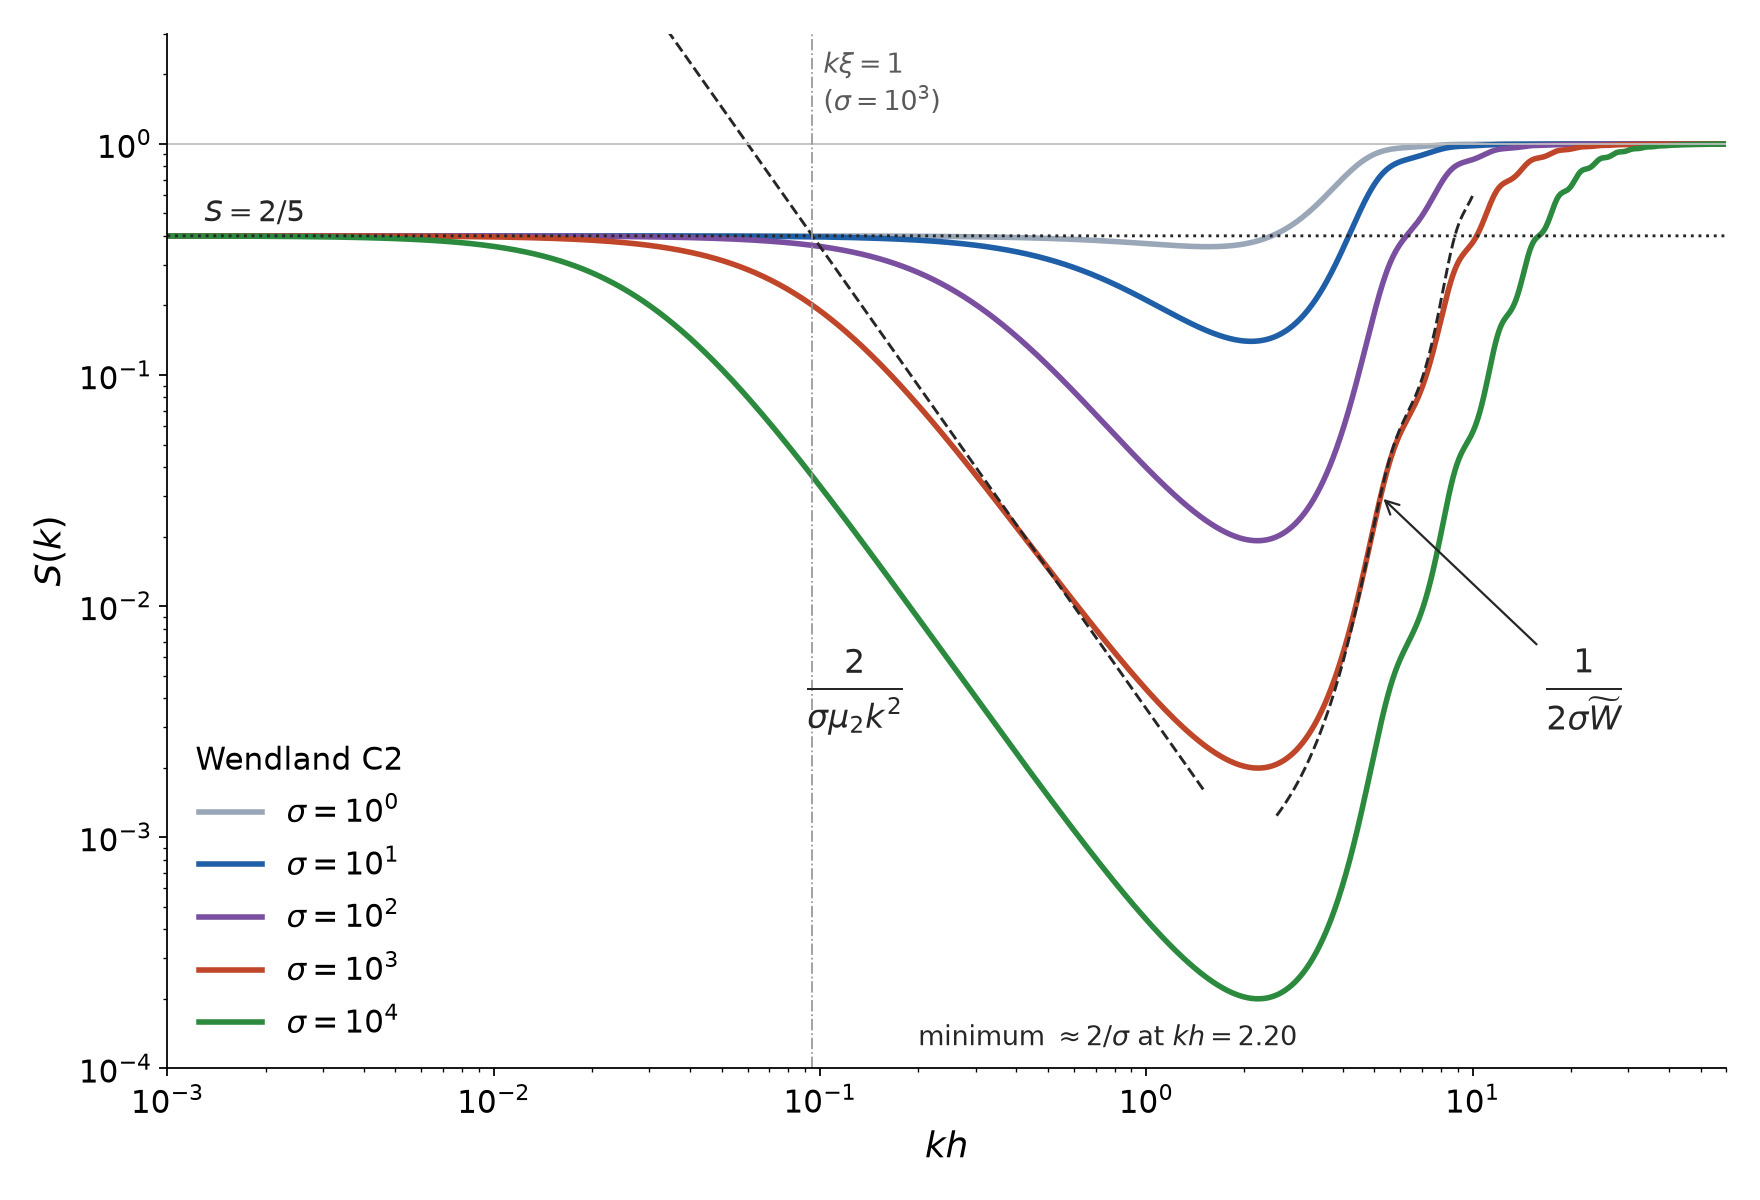
\includegraphics[width=0.7\textwidth]{figs/sk_regimes.png}
\caption{\Eq{Sk} for Wendland C2 at $\sigma=1$--$10^4$; dashed, the asymptotes at $\sigma=10^3$; open circles, $k_*$.  Script: \texttt{examples/sk\_regimes.py}.}
\label{fig:skreg}
\end{figure}

\subsection{The logarithm in two dimensions}
\label{sec:log}

The variance \Eq{Vvar} is dominated by the middle regime, where $\widetilde W\simeq1$ and $S\simeq2/(\sigma\mu_2k^2)$:
\st
\frac{\avg{\delta V_a^2}}{\bar V^2}\simeq\frac1{\bar n}\int_{1/\xi}^{1/h}\frac{d^2k}{(2\pi)^2}\,\frac{2}{\sigma\mu_2k^2}\sim\frac1\pi\,\frac{\ln\sigma}{\sigma\,\bar nh^2} .
\stp
In $d$ dimensions the integrand is $k^{d-3}dk$: the long wavelengths dominate in $d=1$, the kernel scale in $d=3$, and every decade between $h$ and $\xi$
in $d=2$, which is marginal.  A box smaller than $\xi$ cuts the logarithm off.

\subsection{What the fluid sees}
\label{sec:leak}

The point: the fluid fields see the positions only through the kernel, filtered by $1-\widetilde W$, so whatever the points do at long wavelength reaches the
hydrodynamic correlators only at the order of a gradient.

\paragraph{The entropy.}  At fixed positions each particle's entropy is its share of the bath plus an intrinsic fluctuation, \Eq{intrinsic},
\st
s_a=s\,V_a+\delta s_a,\qquad \avg{\delta s_a^2}=C_V\,V_a .
\stp
For the point sum $S_{\bm k}=\sum_as_a\,e^{-i\bm k\cdot\bm x_a}$ the two parts add independently.  The intrinsic part gives $C_V\sum_aV_a\simeq C_VL^2$, whatever the
positions.  The mean part is $s\int d^2x\,(\rho/n)\,e^{-i\bm k\cdot\bm x}$, which to first order in the density modes is $s\,(1-\widetilde W)\,\delta\rho_{\bm k}/\bar n$: the
entropy misplaced because the volumes of the particles do not tile the box.  With $s^2/(\bar nC_V)=c_s^2s_a=(1+c_s^2)\,\sigma$ for a constant $c_s^2=s/C_V$,
\begin{keyeq}
\st
\frac{\avg{|S_{\bm k}|^2}}{L^2C_V}=1+\underbrace{(1+c_s^2)\,\sigma\,\big(1-\widetilde W\big)^2S(k)}_{\text{leak}} .
\label{leak}
\stp
\end{keyeq}
For the smoothed entropy density the mean part is filtered by $\widetilde W(1-\widetilde W)$ instead.

\paragraph{The leak at long wavelength.}  With the Ornstein--Zernike form of $S$ (\Sect{sec:regimes}), written for any stiffness of the labels,
\st
S(k)\simeq\frac{1/(1+\mathcal K)}{1+\xi^2k^2},\qquad \xi^2=\frac{\sigma\mu_2}{2(1+\mathcal K)},\qquad \big(1-\widetilde W\big)^2\simeq\frac{\mu_2^2k^4}{16},
\stp
the leak is
\begin{keyeq}
\st
\text{leak}\simeq(1+c_s^2)\,\frac{\mu_2k^2}8\,\frac{\xi^2k^2}{1+\xi^2k^2}\;\le\;(1+c_s^2)\,\frac{\mu_2k^2}8 .
\label{leakbound}
\stp
\end{keyeq}
\begin{itemize}
\item \emph{The present model}, $1+\mathcal K\simeq5/2$ and $\xi$ of the order of $h$: the leak falls as $k^4$ for $k\xi\ll1$.
\item \emph{Neutral labels}, $1+\mathcal K\to0$ and $\xi\to\infty$, with $S\simeq2/(\sigma\mu_2k^2)$ (\nolinkurl{renormalization_sph.tex}): the leak reaches the bound.
\end{itemize}
The bound is a relative correction of order $\mu_2k^2$, the order of the kernel's own smoothing of the fluid fields, $\widetilde W^2\simeq1-\mu_2k^2/2$.  So even
when the points fluctuate as $1/k^2$, the fluid sees them only as a gradient correction of the size of the discretization error the kernel already makes, and
not at all as $k\to0$.  At the scale of the kernel the leak is of order one whatever the stiffness: there $S\simeq1/(2\sigma\widetilde W(1-\widetilde W))$ and the leak is
$(1+c_s^2)(1-\widetilde W)/(2\widetilde W)$, a property of point sums at $kh\sim1$, not of hydrodynamics.

\paragraph{The momentum.}  At rest each particle's mean momentum is zero, so there is no mean part, and with \Eq{intrinsic}
\st
\frac{\avg{|M_{\bm k}|^2}}{L^2\,T(e+p)}=\avg{V_a}\bar n ,
\label{Mpred}
\stp
flat in $k$, the same for both projections: the positions do not leak into the momentum at all.  The mean volume (\Sect{sec:Vfluct}) stays finite for any
stiffness, since its integrand $\widetilde W(1-\widetilde W)S$ tends to $1/(2\sigma)$ at small $k$ for neutral labels.

%=============================================================================
\section{The positions back in the thermodynamics}
\label{sec:back}

\subsection{The correction to the label pressure and energy}
\label{sec:loopcorr}

The one-loop term of the positions in \Eq{lnZN} depends on $\bar n$ through $\sigma$ (at fixed $h$) and on $T$ through $\sigma$.  Differentiating as in
\Sect{sec:pe},
\begin{keyeq}
\st
\frac{\delta p}T=\frac12\int\frac{d^2k}{(2\pi)^2}\ln S-\sigma\int\frac{d^2k}{(2\pi)^2}\,\widetilde W(1-\widetilde W)\,S,\qquad
\delta e_a=e\,\bar V\,\big(\avg{V_a}\bar n-1\big) .
\label{labelloop}
\stp
\end{keyeq}
Both are negative, of order $1/(\bar nh^2)$ per particle, and grow with $\sigma$ as the stiff band of $S(k)$ widens:
\begin{center}
\begin{tabular}{ccccc}
\toprule
$\sigma$ & $I_0$ & $\sigma I_1$ & $\delta p/\bar nT$ & $\delta e_a/T$ \\
\midrule
3.89 & $-2.03$ & 0.45 & $-0.32$ & $-0.20$ \\
16.4 & $-4.14$ & 1.07 & $-0.68$ & $-0.46$ \\
179 & $-13.43$ & 3.11 & $-2.13$ & $-1.35$ \\
\bottomrule
\end{tabular}
\end{center}
with $I_0=h^2\!\int\!\frac{d^2k}{(2\pi)^2}\ln S$ and $I_1=h^2\!\int\!\frac{d^2k}{(2\pi)^2}\widetilde W(1-\widetilde W)S$ for C2; the last two columns at $h/a=2$
($\bar nh^2=4.62$), against $1+\mathcal K_0=2.5$ and $\Delta e/T=5$.  At $\sigma=3.89$ the positions reduce the label pressure by $13\%$; at $\sigma=179$ by more
than four fifths, where the number of stiff modes per particle is close to one and the Gaussian integral is at the edge of its validity.

\subsection{Consequences for the renormalization}
\label{sec:loopren}

\Eq{labelloop} depends on $\bar nh^2$ as well as on $\sigma$.  Along a curve of fixed $\mu/T$ at fixed $h$ the density changes with $T$, and with it the number of
neighbours: the kernel is a scale, and the conformal form \Eq{Pconf} is broken at order $1/(\bar nh^2)$.  It is measured, not tuned: the plot of $P/T^3$
along fixed $\mu/T$ (\nolinkurl{renormalization_sph.tex}) measures it.

%=============================================================================
\section{Against hybrid Monte Carlo}
\label{sec:hmc}

Hybrid Monte Carlo (\texttt{examples/volume\_fluctuations.jl}, Liouville measure, 200 updates from the lattice, the first third discarded) in a box $L=9h$ at
$h/a=2$, $3$, $4$.

\paragraph{The temperature of the runs.}  The runs start on the lattice, at rest, with the entropy density $S_0$, and sample the canonical ensemble at the
temperature $T_0$ whose mean energy equals that of the start.  Each particle holds the fluctuation energy $\Delta e$ besides its share of the fluid's, so
$T_0$ is below $T(S_0)$:
\st
\frac{T_0}{T(S_0)}=0.855,\ 0.955,\ 0.996,\qquad \sigma(T_0)=3.89,\ 16.4,\ 179\qquad(S_0\bar V=16,\ 54,\ 541) .
\stp
Every constant of the theory is evaluated at $T_0$.  The theory then has no free parameter.

\paragraph{Results.}
\begin{itemize}
\item \emph{The scale is $h$.}  $S(k)$ at $h/a=2$ and $4$ lies on one curve in $kh$ (\Fig{fig:sk}); the hole of $g(r)$ has the same radius in $r/h$ and a
  depth proportional to $1/(\bar nh^2)$ (\Fig{fig:gr}); the volume variance times $\bar nh^2$ is the same at the three $h/a$.
\item \emph{$S(k)$} follows \Eq{Sk} with the exact $\Pi$ and $\mathcal K$ to $0$--$3\%$ over the box modes.  With the one-loop values it is $3$--$8\%$ low at
  $\sigma=3.89$; at the $\sigma$ of the start it would be $19$--$24\%$ low.
\item \emph{The volumes.}  The mean agrees to $0.01$--$0.2\%$, the variance to $0$--$8\%$ (Table~\ref{tab:hmc}); the theory is high at $h/a=2$, where a particle has
  only $4.6$ neighbours.
\item \emph{The fluid variables.}  The momentum correlator is flat in $k$, the same for both projections, at the level of the exact single particle,
  $r_m\avg{V_a}\bar n$, to $1\%$; the positions do not leak into the momentum.
\item \emph{The core.}  At $\sigma=179$ and $h/a=2$ the Gaussian theory gives $g(0)=-0.36$; the particles keep $g\approx0.1$.  The core, $r\lesssim0.3h$, is the one
  place where the theory is qualitative.
\end{itemize}

\begin{table}[h]
\caption{Volumes: hybrid Monte Carlo against the theory with the exact single particle at $\sigma(T_0)$, in the same box.  The variance is normalized by
$\bar V$.  In parentheses, the one-loop $\Pi$ and $\mathcal K$.}
\label{tab:hmc}
\begin{ruledtabular}
\begin{tabular}{ccc cc ccc}
$h/a$ & $S_0\bar V$ & $\sigma(T_0)$ & $\avg{V_a}\bar n$ & theory & $10^3\,\bar n^2\avg{\delta V_a^2}$ & theory & ratio \\
\colrule
2 & 16  & 3.89  & 0.9737(1) & 0.9755 & 16.40(37) & 17.19 (16.26) & 0.95 (1.01) \\
2 & 54  & 16.4  & 0.9855(1) & 0.9864 & 7.33(25)  & 7.99 (7.92)   & 0.92 (0.93) \\
2 & 541 & 178.8 & 0.9959    & 0.9965 & 1.03(4)   & 1.12 (1.12)   & 0.92 (0.92) \\
3 & 16  & 3.89  & 0.9885(1) & 0.9888 & 7.32(9)   & 7.64 (7.23)   & 0.96 (1.01) \\
3 & 54  & 16.4  & 0.9937    & 0.9939 & 3.68(13)  & 3.55 (3.52)   & 1.04 (1.05) \\
3 & 541 & 178.7 & 0.9983    & 0.9984 & 0.50(2)   & 0.50 (0.50)   & 1.00 (1.00) \\
4 & 16  & 3.89  & 0.9935    & 0.9937 & 4.35(11)  & 4.30 (4.07)   & 1.01 (1.07) \\
4 & 54  & 16.4  & 0.9964    & 0.9965 & 1.93(8)   & 2.00 (1.98)   & 0.96 (0.97) \\
4 & 541 & 178.7 & 0.9990    & 0.9991 & 0.29(2)   & 0.28 (0.28)   & 1.04 (1.04) \\
\end{tabular}
\end{ruledtabular}
\end{table}

\begin{figure}[h]
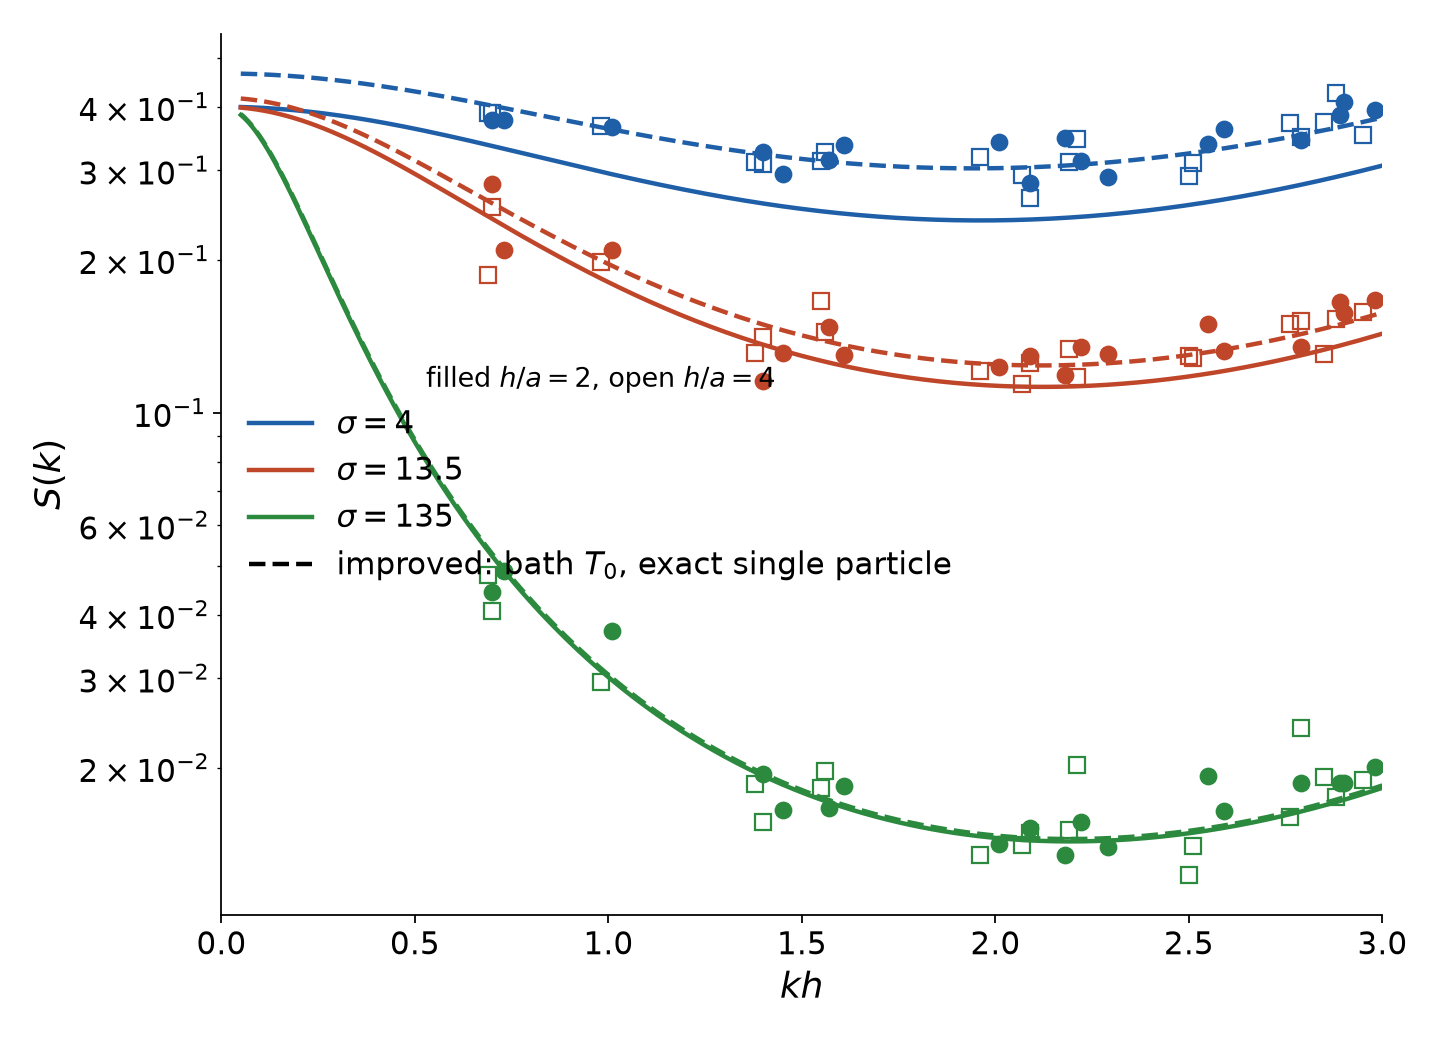
\includegraphics[width=0.7\textwidth]{figs/equilibrium_Sk.png}
\caption{$S(k)$, hybrid Monte Carlo (points), $L=9h$, at $h/a=2$ (filled) and $4$ (open), against \Eq{Sk} with the one-loop (solid) and the exact (dashed)
$\Pi$ and $\mathcal K$ at $\sigma(T_0)$.  One curve per $\sigma$: the theory does not depend on $h/a$.}
\label{fig:sk}
\end{figure}

\begin{figure}[h]
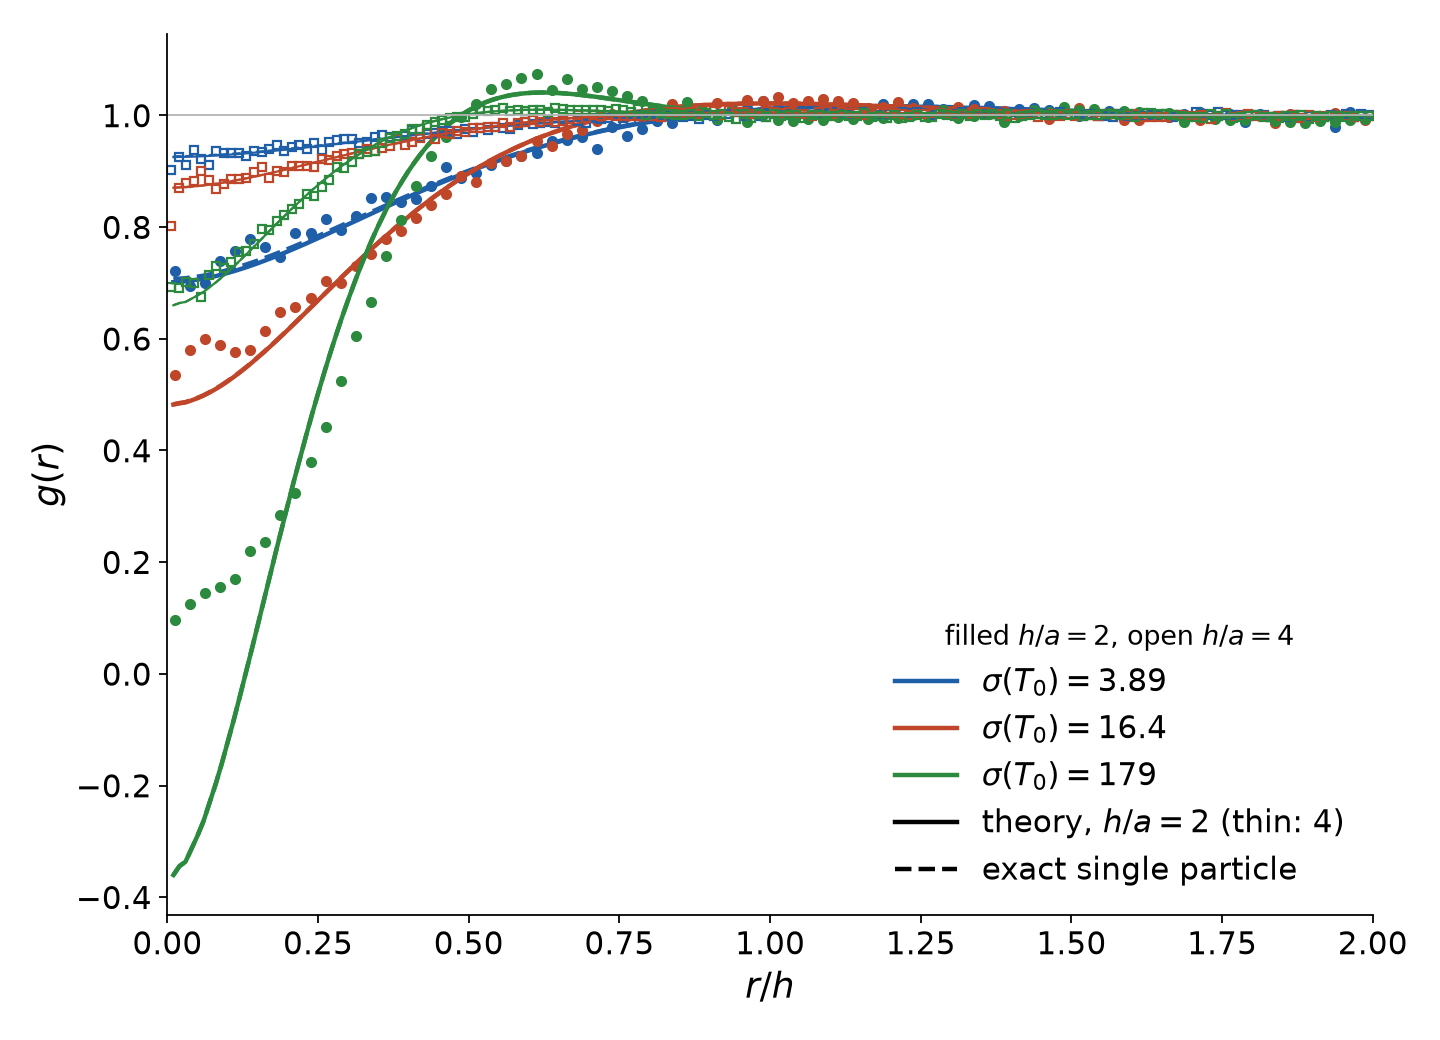
\includegraphics[width=0.7\textwidth]{figs/equilibrium_gr.png}
\caption{$g(r)$, hybrid Monte Carlo (points) at $h/a=2$ (filled) and $4$ (open), against the Gaussian theory with the one-loop (solid) and the exact (dashed)
single particle.}
\label{fig:gr}
\end{figure}

%=============================================================================
\section{Discussion}
\label{sec:discussion}

\paragraph{A window, not a limit.}  The physical continuum limit holds the fluid fixed ($s$, $T$) and the kernel fixed in physical units, and adds particles.
Then the entropy in a kernel, $s\,h^2=s_a\,\bar nh^2$, is fixed, and both $s_a$ and $\sigma$ fall as $1/(\bar nh^2)$.  The two expansions need
\st
1\ll\bar nh^2\ll s\,h^2 ,
\stp
so the limit is $s\,h^2\to\infty$, the kernel holding many quanta, with $\bar nh^2$ in the window.  As $s_a$ falls the cutoff terms of \Sect{sec:pe} grow, as
$T\Lambda^d$ does, and the renormalization of \Sect{sec:ren} becomes necessary rather than a refinement.

\paragraph{An extra slow mode.}  The entropy per particle is a variable of the model that the target fluid does not have.  At fixed $T$ it fluctuates with the
density of labels, and it diffuses through the stochastic step.  Neither a static field nor sound excites it at leading order, and it reaches the stress only
through the label pressure, at order $1/\sigma$; it may show as a small diffusive peak in the longitudinal correlator.

\paragraph{What remains.}
\begin{itemize}
\item The renormalization of the bare equation of state, and its tests (\nolinkurl{renormalization_sph.tex}).
\item Beyond the Gaussian theory of the positions, through $\Gamma[S]$ (\Sect{sec:response}), for the core of $g(r)$.
\end{itemize}

%=============================================================================
\appendix

\section{The single-particle integral beyond one loop}
\label{app:single}

The exponent is $V\psi$, with $V\psi_{\max}$ of order $s_a$.  The cubic and quartic derivatives of $\psi$ at the maximum change $\ln Z_1$ by
\st
\ln Z_1=\frac pTV+\mathcal K_0\ln V+\tfrac12\ln\det(2\pi\chi)+\frac{c}{s\,V}+O\Big(\frac1{s_a^2}\Big),
\stp
with $c$ a number of order one fixed by the equation of state.  The correction depends on $V$, so it enters $\Pi$ and $\mathcal K$; at small $s_a$ the quadrature of
\Sect{sec:quadrature} replaces the series.

\section{The kernels}
\label{app:kernels}

For small $k$,
\st
\widetilde W(k)=1-\frac{\mu_2k^2}{4}+O(k^4),\qquad \mu_2=\int d^2r\,r^2\,W(r),
\stp
the $1/4$ being $1/(2d)$.  For the Wendland kernels $\mu_2/h^2=5/9$, $0.424$, $0.343$ (C2, C4, C6), and $0\le\widetilde W\le1$ at every $k$ (\Fig{fig:wft}), so
every mode of \Eq{Ak} is stable; a kernel with $\widetilde W<0$ somewhere would be unstable there.

\begin{figure}[h]
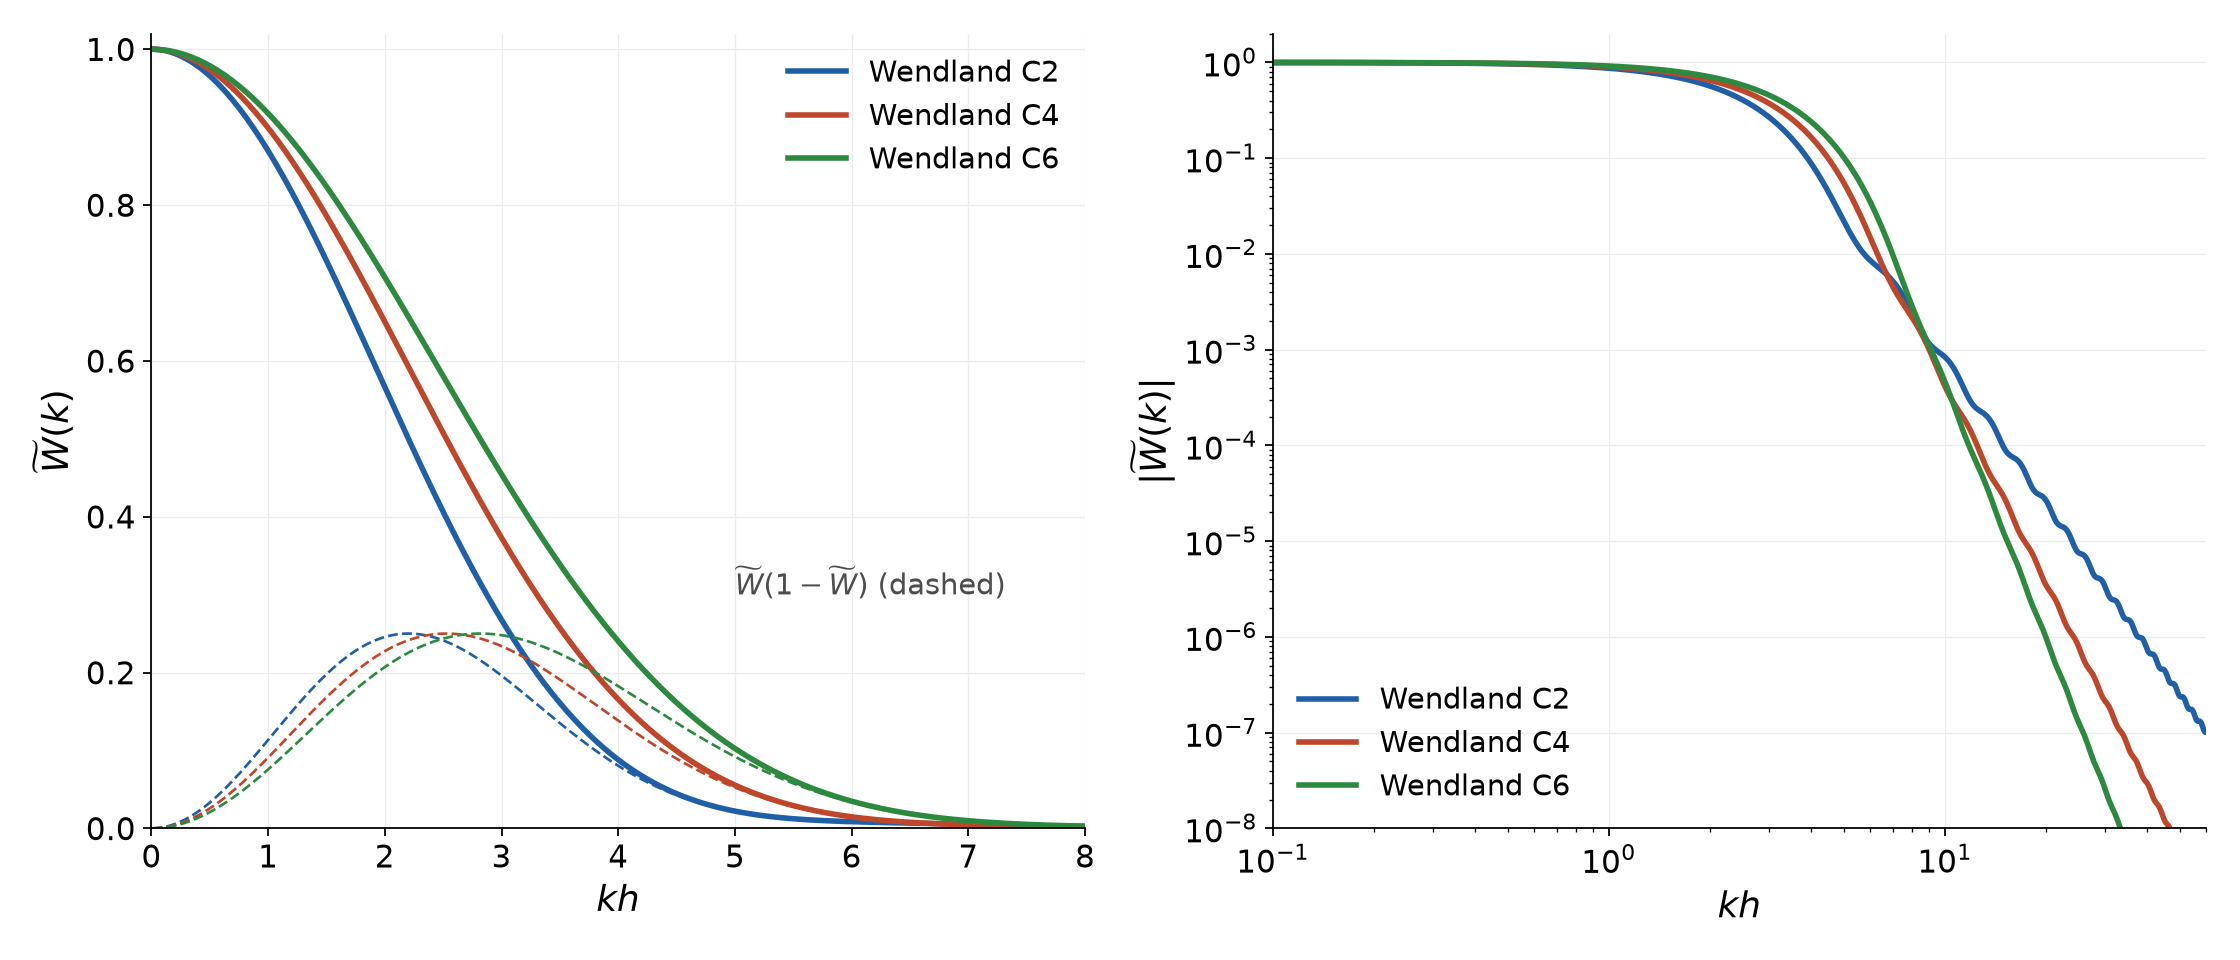
\includegraphics[width=0.6\textwidth]{figs/wendland_ft.png}
\caption{The Fourier transforms of the Wendland kernels.}
\label{fig:wft}
\end{figure}

%=============================================================================
\section{Notes from discussion}
\label{app:notes}

A place for short derivations that come up in discussion, to be moved into the main text or into another note when they settle.

\subsection{The mechanical pressure of a particle and $p_1$: Legendre at tree level, an average exactly}
\label{app:legendre}

The question: is the mechanical pressure of a particle, a function of its microcanonical variables,
\st
p_a(s,\bm m,V)=-\frac{\partial e_a}{\partial V}\Big|_{s,\bm m},
\stp
the same as the pressure of a particle at fixed temperature, $p_1(T,\bm v,V)=-\partial F_1/\partial V$, at corresponding points?

\paragraph{At tree level: a Legendre transform.}  The tree-level free energy is the Legendre transform of the energy over the entropy and the momentum,
\st
F^{\rm tree}(T,\bm v,V)=\min_{s,\bm m}\big[e_a(s,\bm m,V)-Ts-\bm v\cdot\bm m\big] .
\stp
By the envelope theorem the $V$-derivative at fixed $(T,\bm v)$ is the $V$-derivative of $e_a$ at fixed $(s,\bm m)$, at the corresponding point:
\begin{keyeq}
\st
p_1^{\rm tree}(T,\bm v,V)=-\frac{\partial F^{\rm tree}}{\partial V}\Big|_{T,\bm v}=p_a\big(s_*,\bm m_*,V\big),\qquad
\frac{\partial e_a}{\partial s}\Big|_*=T,\qquad \frac{\partial e_a}{\partial\bm m}\Big|_*=\bm v ,
\stp
\end{keyeq}
the familiar $(\partial E/\partial V)_S=(\partial F/\partial V)_T$.  At rest, $\bm v=0$ corresponds to $\bm m_*=0$ and $s_*=s(T)\,V$, and $p_1^{\rm tree}=p(T)$.

\paragraph{Exactly: a canonical average, a Laplace transform.}  The free energy of a particle is $F_1=-T\ln Z_1$, an integral over the entropy and the momentum rather than a
maximum.  The Liouville measure does not depend on $V$, so
\begin{keyeq}
\st
p_1(T,\bm v,V)=-\frac{\partial F_1}{\partial V}\Big|_{T,\bm v}=\avg{p_a}_{T,\bm v,V} ,
\stp
\end{keyeq}
the canonical average of the mechanical pressure at fixed volume.

\paragraph{The average, and why the identity holds.}  The average is over the distribution of one particle's entropy and momentum at a fixed volume,
\st
\avg{\,\cdot\,}_{T,\bm v,V}=\frac1{Z_1}\int ds\,d^d\bm m\;(\,\cdot\,)\;e^{\,s-e_a(s,\bm m,V)/T+\bm v\cdot\bm m/T},\qquad Z_1=\int ds\,d^d\bm m\;e^{\,s-e_a/T+\bm v\cdot\bm m/T} .
\stp
Differentiating under the integral,
\st
p_1=T\,\frac{\partial\ln Z_1}{\partial V}\Big|_{T,\bm v}=\frac T{Z_1}\int ds\,d^d\bm m\;\Big(-\frac1T\frac{\partial e_a}{\partial V}\Big)\,e^{\,s-e_a/T+\bm v\cdot\bm m/T}=\avg{p_a}_{T,\bm v,V} .
\stp
This needs the measure $ds\,d^d\bm m$ and the limits of integration not to depend on $V$, which holds for the Liouville measure, flat in $s$ and $\bm m$.  It fails for a
measure that depends on $V$: the Einstein measure, flat in $e$, carries the Jacobian $\partial s/\partial e=1/T_a(s,\bm m,V)$, and then
\st
p_1=\avg{p_a}+T\,\Big\langle\frac{\partial\ln(1/T_a)}{\partial V}\Big\rangle ,
\stp
a difference of order $1/s_a$ (the Einstein measure gives $\avg{p_aV/T_a}$ in place of $\avg{p_a}V/T$).

\paragraph{In the full ensemble} the volume fluctuates as well, and the average of $p_a$ is the conditional average averaged over $V_a$,
\st
\avg{p_a}_{\rm ens}=\big\langle p_1(T,V_a)\big\rangle_{V_a}\simeq p_1(T,\bar V)+\tfrac12\,\frac{\partial^2p_1}{\partial V^2}\,\avg{\delta V_a^2}+\dots ,
\stp
and the stress operator carries the factor $V_a^2Q_a^{ii}$, which is correlated with $V_a$.  These correlations are where the correction of the positions, of order
$1/(\bar nh^2)$, enters the measured pressure.  The identity $p_1=\avg{p_a}$ is exact conditionally, at fixed volume.

\paragraph{The fluctuation share.}  The average differs from the value at the saddle point by the fluctuations; at one loop, at rest,
\st
p_1=\underbrace{p_a(s_*,0,V)}_{p(T)}+\mathcal K_0\,\frac TV+O\Big(\frac T{V s_a}\Big),
\stp
from \Eq{lnZ1} and \Eq{PiK}.  The fluctuation share $\mathcal K_0T/V$ is the difference between the Laplace and the Legendre transforms, and it vanishes relative to
$p$ as $s_a\to\infty$, where the saddle point becomes exact.

\paragraph{What is measured.}  The stress the code measures (\texttt{gravity.tex}) contains $p_a$ particle by particle, $V_aT_a^{ij}=v_a^im_a^j+p_aV_a^2Q_a^{ij}$.  Its
average is $\avg{p_a}=p_1$ (with the closure $Q_a^{ii}\simeq d\,n_a$), and the kinetic stress adds the label term,
\st
p_{\rm model}=\bar nT+\avg{p_a}=\bar nT+p_1 ,
\stp
which holds up to the fluctuations of the volumes: the second equality takes $p_1$ at the mean volume, and the fluctuations of $V_a$ and their correlation with
$V_a^2Q_a^{ii}$ add the correction of the positions, of order $1/(\bar nh^2)$, as in the previous paragraph.  So the measured pressure is the Laplace version, with both one-loop pieces: the label gas $\bar nT$ and the fluctuation share $\mathcal K_0\bar nT$.  These are the pieces
the renormalized Hamiltonian of \nolinkurl{partition_v2.tex} removes.

\subsection{The double Legendre transform in motion, and a shift in \texorpdfstring{$\bm m$}{m}}
\label{app:doublelegendre}

The question: the renormalized Hamiltonian shifts only the entropy variable, $e(s+\Delta s(u),\bm m,V)$, yet in a moving equilibrium it also renormalizes the
momentum.  How, and what is left?  (Theory of the moving case: \nolinkurl{partition_v2.tex}, ``Equilibrium in motion''.)

\paragraph{The double transform.}  At fixed $V$ the free energy of a particle is the Legendre transform over both $s$ and $\bm m$,
\st
F(T,\bm v,V)=\min_{s,\bm m}\big[e(s,\bm m,V)-Ts-\bm v\cdot\bm m\big],\qquad
\frac{\partial e}{\partial s}\Big|_*=T,\qquad \frac{\partial e}{\partial\bm m}\Big|_*=\bm v .
\stp
The small-increment theorem holds for all variables at once: a change of the energy function at fixed $(s,\bm m)$ changes $F$ at fixed $(T,\bm v)$ by the same amount,
evaluated at the saddle $(s_*,\bm m_*)(T,\bm v,V)$,
\st
\delta F\big|_{T,\bm v}=\delta e\big|_{s,\bm m}\Big|_*,\qquad \frac{\delta F}T=\Delta s\big|_*\quad\text{for the entropy shift} .
\stp

\paragraph{Why the shift in $s$ alone moves the momentum.}  The counterterm $\Delta s(u)$ is evaluated at the saddle, where the entropy of the particle is
\st
u_*=\gamma\,s(T_{\rm rel})\,V .
\stp
So $\delta F/T=\Delta s(u_*)$ depends on $\bm v$ through $\gamma$, and the momentum $M=-\partial F/\partial v$ (per particle) gains $-T\,\partial_v\Delta s(u_*)$.  For the conformal
shift, $\Delta s=\tfrac\alpha2\ln u$,
\st
\Delta s(u_*)=\tfrac\alpha2\big(1+1/c_s^2\big)\ln\gamma+\dots=c_\gamma\ln\gamma+\dots,\qquad c_\gamma=\tfrac12(d+1)(3+1/c_s^2)\quad(d\,c_s^2=1) ,
\stp
the $\gamma$ part of the determinant of the boosted susceptibility, which it cancels: the momentum is renormalized through the dependence of the saddle on $\bm v$,
without touching $\bm m$.

\paragraph{What a function of $u$ cannot do.}  At fixed $V$, $u_*$ depends on $(T,\bm v)$ only through one combination,
\st
u_*\propto\gamma^{1+1/c_s^2}\,T^{1/c_s^2}\,V .
\stp
So a shift that depends on $u$ alone can cancel only the parts of the one-loop term that depend on $(T,\bm v)$ through that combination.  The other factor of the
determinant,
\st
\tfrac12\ln\big(1-c_s^2v^2\big) ,
\stp
depends on $v$ separately, and no $\Delta s(u)$ cancels it: it is the momentum left over, $-T v\,c_s^2/(1-c_s^2v^2)$ per particle, and the violation $R$ of the Lorentz
identity.

\paragraph{The general counterterm.}  At fixed $V$ the map $(s,\bm m)\leftrightarrow(T,\bm v)$ is one to one, so any desired $\delta F/T(T,\bm v,V)$ is produced by some function
$\Delta s(s,\bm m,V)$ on the phase space of the particle.  The natural, covariant choice is the determinant evaluated at the particle's own thermal vector, its own
temperature $T_a$ and velocity $\bm v_a$,
\begin{keyeq}
\st
\Delta s_a=\ln\Big[V_a^{\,1-\mathcal B}\,\det\big(2\pi V_a\,\chi^{\mu\nu}(T_a,\bm v_a)\big)^{1/2}\Big]-\ln T_a+\text{const} ,
\stp
\end{keyeq}
the moving generalization of the shift of \nolinkurl{partition_v2.tex}.  At the saddle it cancels the whole one-loop term, the factor $1-c_s^2v^2$ included, and at one
loop restores
\st
M=w\gamma^2v,\qquad M=v\,\big(T^{00}+T^{yy}\big) .
\stp
Equivalently one could shift the momentum variable, $e(s,\bm m+\Delta\bm m,V)$, which changes $F$ by $\bm v\cdot\Delta\bm m$ at the saddle.

\paragraph{The price.}
\begin{itemize}
\item A dependence on $\bm m$ changes the ideal dynamics: the velocity becomes
  \st
  \dot{\bm x}_a=\frac{\partial e}{\partial\bm m}\Big|_u+T_a\,\frac{\partial\Delta s}{\partial\bm m} ,
  \stp
  a correction of relative order $1/s_a$, a momentum counterterm.
\item A dependence on $V$ at fixed $(s,\bm m)$ adds a force term (the pressure of the counterterm).
\item The present shift, in $u$ only, changes neither.  It renormalizes all that a function of $u$ can reach, and leaves exactly the $1-c_s^2v^2$ piece: the phase space of
  the foliation dependence of the sound mode, the stiffness on the moving adiabat.
\end{itemize}
So the last piece is removed by a shift that depends on $\bm m$, at the price of a small velocity correction.  (Correction, 2026-11-22: a comoving volume alone would
not remove it.  The factor $1-c_s^2v^2$ is the foliation dependence of the susceptibility itself, the sound stiffness on the moving adiabat, as in the Density Frame
paper; see \nolinkurl{partition_v2.tex}, ``The counterterms: formal structure''.)

\subsection{The quadratic form in motion: sound waves and the density-frame condition}
\label{app:soundmodes}

The question (2026-11-22): the counterterm $\delta\ln Z_{1,a}$ must be split between the entropy and the momentum, $\Delta s_a+\bm v_a\cdot\Delta\bm m_a/T_a=\delta\ln Z_{1,a}$
(\nolinkurl{partition_v2.tex}, ``The counterterms: formal structure'').  How should the split be made?  This needs the quadratic form of a particle's fluctuations and
its origin.  Two ways to organize it, which agree: by the normal modes (the sound waves), and by which terms violate the density-frame condition.

\paragraph{The quadratic form.}  The Gaussian weight of a particle's fluctuations is
\st
\exp\Big[-\tfrac V2\,\delta\beta_\mu\,\chi^{\mu\nu}\,\delta\beta_\nu\Big],\qquad \chi^{\mu\nu}=n_\lambda\,\mathcal X^{\lambda\mu\nu},\qquad
\mathcal X^{\lambda\mu\nu}=\frac{\partial T^{\lambda\mu}}{\partial\beta_\nu},
\stp
with $n$ the lab time direction.  The quadratic form
\st
S^\lambda\equiv\mathcal X^{\lambda\mu\nu}\,\delta\beta_\mu\,\delta\beta_\nu
\stp
is the second-order entropy current of the fluctuations, conserved by the linearized ideal equations, and the weight is its flux through the lab slice, $V\,n_\lambda S^\lambda$.
Write the fluctuation of the thermal vector in the rest-frame variables,
\st
\delta\beta_\mu=\delta\beta_{\rm rel}\,u_\mu+\beta_{\rm rel}\,\delta u_\mu ,
\stp
and split $\delta\bm u$ along and across the flow, $\delta u_\parallel$, $\delta\bm u_\perp$.  With the rest-frame components of $\mathcal X$
($\mathcal X^{\hat0\hat0\hat0}=wT_{\rm rel}/c_s^2$, $\mathcal X^{\hat0\hat\imath\hat\jmath}=wT_{\rm rel}\delta^{ij}$ and permutations) and $n=\gamma(1,\bm v)$ in the rest frame,
\st
\delta\beta_\mu\chi^{\mu\nu}\delta\beta_\nu=\gamma\,wT_{\rm rel}\beta_{\rm rel}^2\Big[a^2+2c_sv\,a\,\delta u_\parallel+\delta u_\parallel^2+\delta\bm u_\perp^2\Big],\qquad
a\equiv\frac{\delta\beta_{\rm rel}}{c_s\beta_{\rm rel}}=-\frac{\delta p}{w\,c_s} ,
\stp
with $\delta p=s\,\delta T_{\rm rel}=w\,\delta T_{\rm rel}/T_{\rm rel}$.  The lab slice couples the temperature and the longitudinal velocity through $v$; nothing else is coupled.

\paragraph{The normal modes.}  The $2\times2$ block is diagonal in
\st
J_\pm=a\pm\delta u_\parallel ,
\stp
the two sound waves (Riemann combinations of $\delta p/(wc_s)$ and $\delta u_\parallel$) running along and against the flow:
\begin{keyeq}
\st
\delta\beta_\mu\chi^{\mu\nu}\delta\beta_\nu=\gamma\,wT_{\rm rel}\beta_{\rm rel}^2\Big[\tfrac12(1+c_sv)\,J_+^2+\tfrac12(1-c_sv)\,J_-^2+\delta\bm u_\perp^2\Big] .
\label{modesform}
\stp
\end{keyeq}
Each mode $m$ is weighted by
\st
\gamma\,(1+v\,w_m),\qquad w_m=+c_s,\ -c_s,\ 0\ (\text{the }d-1\text{ transverse modes}),
\stp
$w_m$ its velocity along the flow in the rest frame.  This is the flux statement above: in the rest frame each mode's entropy current is $S^x=w_mS^0$ (for $J_\pm$,
$2c_s\,a\,\delta u_\parallel/(a^2+\delta u_\parallel^2)=\pm c_s$; for $\delta\bm u_\perp$, $S^x=0$), and the lab slice measures
\st
n_\lambda S^\lambda=\gamma\big(S^0+vS^x\big)=\gamma\,(1+v\,w_m)\,S^0 .
\stp
The product of the weights is $\gamma^{d+1}(1-c_s^2v^2)$, the determinant of \nolinkurl{partition_v2.tex}.  So the one-loop term is a sum over modes,
\st
\tfrac12\ln\det\big(2\pi V\chi\big)-\ln T=\underbrace{\mathcal K_0\ln(\gamma V)+\ln\gamma+\Lambda(T_{\rm rel})}_{\text{every mode: }\gamma\text{, and the rest frame}}
+\underbrace{\tfrac12\ln(1+c_sv)+\tfrac12\ln(1-c_sv)}_{\text{the sound waves: }1+vw_m} .
\stp
The factor $\gamma$ of each mode is the length contraction, common to all; the factor $1+vw_m$ is the Doppler factor of a mode that moves, and only the sound waves move.

\paragraph{The density-frame condition as a linear condition on $\ln Z_1$.}  Per particle, with $\ln\mathcal Z_N=N\,g(\beta_\mu,\bar V)$ at fixed $N$, the energy and
momentum per particle are $E=\partial g/\partial\beta_0$, $\bm P=\partial g/\partial\bm\beta$, and the pressure times the volume $p\bar V=T\,\bar V\partial g/\partial\bar V$.
The ideal (density-frame) relation $\bm P=\bm v\,(E+p\bar V)$ is linear in $g$; define its violation
\st
\mathcal D[g]\equiv P_\parallel-v\,\big(E+p\bar V\big) .
\stp
Two results, by direct differentiation with $\beta_{\rm rel}=\sqrt{\beta_0^2-\bm\beta^2}$, $\gamma=|\beta_0|/\beta_{\rm rel}$:
\begin{itemize}
\item $\mathcal D[g]=0$ for every function of the two invariants of a particle, its rest-frame temperature and its rest-frame volume,
  \st
  g=g\big(\beta_{\rm rel},\,V_{\rm rest}\big),\qquad V_{\rm rest}=\gamma\bar V .
  \stp
  (For $f(\beta_{\rm rel})$: $\bm P=\bm vE$ and $p=0$.  For $h(V_{\rm rest})$ the energy, the momentum and the pressure combine to zero.  $\ln\gamma$ alone is not of this form:
  it gives $\mathcal D=Tv$, which the label term $\ln\bar V$, with $\mathcal D=-Tv$, cancels; only $\ln(\gamma\bar V)$ is invariant.)
\item For a function of the velocity at fixed $T_{\rm rel}$ and $V_{\rm rest}$,
  \st
  \mathcal D[g]=T\,(1-v^2)\,\frac{\partial g}{\partial v} .
  \stp
\end{itemize}
So every term of $\delta\ln Z_{1,a}$ is either invariant, and respects the density frame, or violates it, and the violating part is defined without ambiguity as
\st
\delta\ln Z_1^{\rm viol}\equiv \delta\ln Z_1\big(\beta_{\rm rel},V_{\rm rest},v\big)-\delta\ln Z_1\big(\beta_{\rm rel},V_{\rm rest},0\big) ,
\stp
the dependence on the velocity at fixed invariants.  At one loop it is the sound term, mode by mode:
\begin{keyeq}
\st
\delta\ln Z_1^{\rm viol}=\sum_{\pm}\tfrac12\ln(1\pm c_sv),\qquad \mathcal D\big[\tfrac12\ln(1\pm c_sv)\big]=\pm\,\frac{c_s\,T\,(1-v^2)}{2\,(1\pm c_sv)} ,
\label{Dviol}
\stp
\end{keyeq}
each sound wave violating the density frame by its own Doppler term, the two cancelling at $v=0$.  Their sum, $-c_s^2vT(1-v^2)/(1-c_s^2v^2)$, divided by the momentum
$w\gamma^2v\bar V$, is $R$.  The transverse modes and the entropy (label) mode do not move, and do not violate it.  (With $c_s^2$ depending on $T_{\rm rel}$ the formulas hold
at fixed $T_{\rm rel}$, which is how $\delta\ln Z_1^{\rm viol}$ is defined.)

\paragraph{The split.}  This suggests the split by the density-frame condition:
\st
\Delta s_a=\delta\ln Z_{1,a}-\delta\ln Z^{\rm viol}_{1,a}\quad(\text{a function of }T_{{\rm rel},a},\ \gamma_aV_a),\qquad \bm v_a\cdot\Delta\bm m_a=T_a\,\delta\ln Z^{\rm viol}_{1,a} .
\stp
The entropy shift is then a function of the particle's invariants, and the momentum shift carries exactly what violates the density frame.  It is the conjugate split
of \nolinkurl{partition_v2.tex}, now with a definition: the invariant part is what $\mathcal D$ annihilates.  Mode by mode the momentum shift is the momentum of the two
sound waves on the lab slices,
\st
\Delta m_{a,\parallel}=\frac{T_a}{2v_a}\Big[\ln(1+c_sv_a)+\ln(1-c_sv_a)\Big]=\frac{T_a}{2v_a}\ln\big(1-c_s^2v_a^2\big) ,
\stp
the sum of the two waves (the logarithm of the product of their Doppler factors, not of their ratio), which is \nolinkurl{partition_v2.tex}'s $\Delta\bm m$.  The momentum
that each wave contributes to the particle is
\st
T\,\partial_v\tfrac12\ln(1\pm c_sv)=\pm\frac{c_sT}{2(1\pm c_sv)} ,
\stp
equal and opposite at rest, and unbalanced in motion by the Doppler factors; the sum is $-c_s^2vT/(1-c_s^2v^2)$.  The ratio appears in the difference of the two waves,
$\tfrac12\ln[(1+c_sv)/(1-c_sv)]={\rm artanh}(c_sv)$, odd in $v$, which cancels in the sum.  The other splits are other ways of factorizing the $2\times2$ block; see the next paragraph.

\paragraph{Three factorizations of the sound block.}  Drop the common factor $\gamma\,wT_{\rm rel}\beta_{\rm rel}^2$ and write $b\equiv\delta u_\parallel$.  The block of
\Eq{modesform} is
\st
Q(a,b)=a^2+2c_sv\,ab+b^2 ,\qquad \det Q=1-c_s^2v^2 .
\stp
Its Gaussian integral is fixed, $\int da\,db\,e^{-VQ/2}\propto(1-c_s^2v^2)^{-1/2}$, but there are three natural ways to say which fluctuation carries the factor.
\begin{enumerate}
\item \emph{Velocity first (the sound factor on the thermometer).}  Complete the square in $b$:
  \st
  Q=\big(b+c_sv\,a\big)^2+\big(1-c_s^2v^2\big)\,a^2 .
  \stp
  At fixed $a$ the velocity fluctuates about $-c_sv\,a$ with the rest-frame stiffness $1$: a pressure fluctuation on the lab slice drags a velocity fluctuation with it,
  as in a sound wave.  What is left, the marginal of $a$, has the stiffness $1-c_s^2v^2$: the temperature (or pressure) fluctuations seen on the lab slice are larger by
  $1/(1-c_s^2v^2)$, and in the variable $\delta\beta_{\rm rel}$ the stiffness is
  \st
  \frac{1-c_s^2v^2}{c_s^2}\;\propto\;\frac1{\gamma^2(dP/dE)_{M^i/S}} ,
  \stp
  the pressure derivative on the moving adiabat of \nolinkurl{partition_v2.tex}, which is written in this order: the momentum integrated first, the sound stiffness on the
  energy.  The factor then belongs to the variable conjugate to $T$: the sound term goes into $\Delta s$.
\item \emph{Temperature first (the sound factor on the speedometer).}  Complete the square in $a$:
  \st
  Q=\big(a+c_sv\,b\big)^2+\big(1-c_s^2v^2\big)\,b^2 .
  \stp
  At fixed velocity the temperature fluctuates about $-c_sv\,b$ with the stiffness $1$; the marginal of the longitudinal velocity has the stiffness $1-c_s^2v^2$: the
  inertia measured on the lab slice, at fixed energy, is reduced by $1-c_s^2v^2$.  The factor belongs to the variable conjugate to $\bm v$: the sound term goes into $\Delta\bm m$.
  This is the conjugate split of \nolinkurl{partition_v2.tex}.
\item \emph{The normal modes (the two sound waves).}  Diagonalize instead of triangularizing: $Q=\tfrac12(1+c_sv)J_+^2+\tfrac12(1-c_sv)J_-^2$.  No variable is integrated first;
  each wave carries its own Doppler factor and its own term $\tfrac12\ln(1\pm c_sv)$.  Each $J_\pm$ is half temperature and half velocity, so this factorization does not by
  itself say $\Delta s$ or $\Delta\bm m$; the density-frame criterion does, since each $\tfrac12\ln(1\pm c_sv)$ depends on $v$ at fixed invariants: both go into $\Delta\bm m$.  One
  wave alone would give $\Delta m_\pm=\pm c_sT/2+O(v)$, a momentum that does not vanish at rest; only the pair is isotropic, the odd parts $\pm{\rm artanh}(c_sv)$ cancelling.
\end{enumerate}

\paragraph{What is the same and what differs.}  The two marginals are equally enhanced: the inverse of $Q$ is
\st
Q^{-1}=\frac1{1-c_s^2v^2}\begin{pmatrix}1&-c_sv\\-c_sv&1\end{pmatrix},\qquad \avg{a^2}\propto\avg{b^2}\propto\frac1{1-c_s^2v^2} ,
\stp
so the statistics do not prefer the temperature or the velocity.  The determinant is the product of the stiffness of the variable integrated first and the Schur
complement of the other, and which is called which is the order of integration.  At one loop every order gives $\tfrac12\ln(1-c_s^2v^2)$ in $\ln Z_1$, and by the
small-increment theorem only $T\Delta s+\bm v\cdot\Delta\bm m$ at the saddle enters; so the three agree on the thermodynamics.  They differ in what the counterterm depends
on across the particle's fluctuations: a $\Delta s$ that depends on $v$ is felt through $\partial\Delta s/\partial\bm m$ in the velocity of the particle, a $\Delta\bm m$
through the inertia.  Those differences enter the Hamiltonian flow, and the equilibrium only at the next order in $1/s_a$.

What decides is not the Gaussian integral but a property of the result: the term violates the density frame, and the density frame is a statement about the momentum.
That selects the second (or, wave by wave, the third), and leaves the entropy shift a function of the invariants.

\paragraph{On $\delta s$ and $\delta p$.}  For one particle at fixed $V$ and no charge there is one thermodynamic variable: $\delta s$, $\delta p$ and $\delta T_{\rm rel}$ are
proportional, and the independent pair is $(\delta p,\delta u_\parallel)$, whose Riemann combinations are $J_\pm$.  A second thermodynamic variable appears only when $V$
fluctuates (the positions): then the entropy per particle and $\delta p$ are independent, as in the Landau--Lifshitz theory of fluctuations, and the entropy per particle is
the non-propagating entropy mode, $w_m=0$, which is where the labels live.  It does not move, so it does not violate the density frame.

\subsection{The velocity near the light cone}
\label{app:velocity}

The question (2026-11-22): we want the velocity of a particle, $\dot{\bm x}=\partial H/\partial\bm m$, to stay below $1$.  Does the split of the counterterm between $\Delta s$
and $\Delta\bm m$ matter?  Script: \nolinkurl{examples/renorm_velocity.py} (conformal fluid, $d=2$, one particle, $V=1$).

\paragraph{What is guaranteed.}  At the saddle point every scheme has $\dot{\bm x}=\bm v$, the velocity of the bath, since the saddle condition of the weight
$\exp[s-(e-\bm v\cdot\bm m)/T]$ in the code's variables is $\partial H/\partial\bm m=\bm v$.  The bound is a property of the whole phase space: $|\partial H/\partial\bm m|<1$
everywhere.  The target energy has it.  With the shift in $u$ alone it holds exactly, since $\dot{\bm x}$ is the target velocity at $(u,\bm m)$.

\paragraph{The check.}  At fixed code entropy $s$, as the momentum grows, compare $1-\dot x$ with $1-v$, $v$ the target velocity at $(u,\bm m)$, $u=s+\tfrac\alpha2\ln s$
(a common reference for all schemes):
\begin{center}
\small
\begin{tabular}{lcccc}
\toprule
$(1-\dot x)/(1-v)$ at $v\to1$ & $u$ only & all in $\Delta s$ & split, sound in $\Delta\bm m$ & $(1+\mathcal K_0)\ln\gamma$ also in $\Delta\bm m$ \\
\midrule
$s=5$ & $1$ & $0.79$ & $0.99$ & leaves the domain \\
$s=16$ & $1$ & $0.91$ & $0.985$ & $0.4$--$0.5$ \\
$s=54$ & $1$ & $0.97$ & $0.985$ & $0.74$ \\
$s=541$ & $1$ & $0.996$ & $0.997$ & $0.987$ \\
\bottomrule
\end{tabular}
\end{center}
\begin{itemize}
\item \emph{All in $\Delta s$} and \emph{the density-frame split}: $\dot x<1$ everywhere, with $1-\dot x$ a fixed fraction $1-O(1/u)$ of $1-v$, the same at every $\gamma$.  The
  reason is that the sound term is bounded, $|\ln(1-c_s^2v^2)|\le|\ln(1-c_s^2)|$, since $c_s<1$: neither shift grows near the light cone.
\item \emph{Moving $(1+\mathcal K_0)\ln\gamma$ into $\Delta\bm m$} (with $-(1+\mathcal K_0)\ln\gamma$ in $\Delta s$): both shifts grow like $\ln\gamma$, the particles move closer to the light
  cone, and at small $s$ the shifted entropy $u-(1+\mathcal K_0)\ln\gamma$ leaves the domain.  It does not help.  (An earlier remark in the discussion, that this split drags fast
  particles, compared the schemes at different reference states and was wrong.)
\end{itemize}

\paragraph{What the density frame says.}  The violating part $\delta\ln Z_1^{\rm viol}$ is bounded uniformly in $v$, so $\Delta\bm m=T\,\delta\ln Z_1^{\rm viol}/v$ is bounded and vanishes linearly at rest;
what grows like $\ln\gamma$ is invariant, $\ln V_{\rm rest}=\ln(\gamma V)$, and stays in the entropy, where for the conformal fluid it is absorbed in $\ln u$ with no velocity term.
For a general equation of state its velocity term is proportional to
\st
\frac{\partial\Delta s}{\partial\ln V_{\rm rest}}\Big|_s=(1+\mathcal K_0)-c_s^2\,T\frac{d\Lambda}{dT}=\mathcal N ,
\stp
the non-conformality.  So the split by the density frame is also the one in which nothing in the counterterm grows near the light cone, apart from the invariant
$\mathcal N\ln V_{\rm rest}$.  Velocity control beyond that (a drag at large $\gamma$) would be a regulator of the dynamics, not part of the renormalization.

\subsection{The label \texorpdfstring{$s_{\rm eff}$}{s\_eff}, the measure and the Hamiltonian, step by step}
\label{app:seff}

The question (2026-11-22): the counterterm can be written as a shift of the entropy argument, or as log terms in the weight, or as an energy added to the
Hamiltonian.  Which variable does the code store, and what goes where?  Notation: $\delta\ln Z_1$ is the excess of a particle's $\ln Z_1$ over the target's
(\nolinkurl{partition_v2.tex}), and the old name $u$ of \texttt{SPH\_RENORM} is $s_{\rm eff}$ below.

\paragraph{Step 1: the model with a shifted argument.}  Each particle carries a label $s$, its entropy variable; the measure is flat in $s$ (Liouville), and the energy is
the target's at a shifted entropy,
\st
H=\sum_a e_{\rm t}\big(s_a+\Delta s_a,\ \bm m_a,\ V_a\big),\qquad \Delta s=\delta\ln Z_1\ \text{at this order} .
\stp
The weight of a particle at the bath temperature $T$ and velocity $\bm v$ is
\st
e^{\,s}\,ds\;\exp\Big[-\frac{e_{\rm t}(s+\Delta s,\bm m,V)-\bm v\cdot\bm m}{T}\Big] .
\stp

\paragraph{Step 2: change the integration variable.}  At fixed $(\bm m,V)$ let
\st
s_{\rm eff}\equiv s+\Delta s ,
\stp
the argument of the target energy.  This is only a change of variables in the integral, so it changes nothing.  In the new variable the energy is the target's,
$e_{\rm t}(s_{\rm eff},\bm m,V)$, with no log terms, and the log terms move into the weight:
\st
e^{\,s}\,ds=\exp\Big[s_{\rm eff}-\Delta s+\ln J\Big]\,ds_{\rm eff},\qquad J\equiv\frac{\partial s}{\partial s_{\rm eff}}\Big|_{\bm m,V}=1-\frac{\partial\Delta s}{\partial s_{\rm eff}}\Big|_{\bm m,V} .
\stp
Two log terms: $-\Delta s$, of order $\ln s$, from $e^{\,s}$; and $\ln J$, of order $1/s$, from the Jacobian.

\paragraph{Step 3: what the flow does to the weight.}  The ideal step is a Hamiltonian flow: the positions and momenta are canonical pairs, and the labels have no conjugate,
so the flow conserves every label (they are Casimirs), and by Liouville's theorem it preserves $\prod_a d\bm x_a\,d\bm m_a$.  It also conserves $H$ and the total momentum.
Hence a weight of the form
\st
f\big(\text{labels}\big)\,\exp\Big[-\frac{H-\bm v\cdot\bm P}T\Big]
\stp
is stationary under the flow, for any function $f$ of the labels.  A weight factor that depends on $\bm m$ or on $V$ (through the positions) is not.

\paragraph{Step 4: split the log terms.}  Write the shift as the part that depends on the label alone and the rest,
\st
\Delta s=\Delta s^{\rm lab}(s_{\rm eff})+\Delta s^{\rm dyn}(s_{\rm eff},\bm m,V) .
\stp
For the conformal fluid $\Delta s^{\rm lab}=\tfrac\alpha2\ln s_{\rm eff}$ (the present \texttt{SPH\_RENORM}) and $\Delta s^{\rm dyn}=\tfrac12\ln(1-c_s^2v^2)$, the sound term; for a general
equation of state $\Delta s^{\rm dyn}$ also contains the dependence on the rest-frame volume $\gamma V$, with the coefficient $\mathcal N$.
\begin{itemize}
\item \emph{The label part stays in the measure.}  $e^{-\Delta s^{\rm lab}}J^{\rm lab}$ is a function of the label, so by Step 3 the flow with the target energy preserves it.  This
  is why \texttt{SPH\_RENORM} works with the target forces unchanged.
\item \emph{The dynamical part goes into the Hamiltonian.}  $e^{-\Delta s^{\rm dyn}}$ depends on $\bm m$ and $V$, so it cannot stay in the weight.  At the saddle the bath
  temperature is the particle's, so
  \st
  e^{-\Delta s^{\rm dyn}}=\exp\Big[-\frac{T_a\,\Delta s^{\rm dyn}}T\Big]\Big(1+O\big(1/s_a\big)\Big) ,
  \stp
  an energy $T_a\Delta s^{\rm dyn}$ in the Boltzmann factor, which can be put into $H$.
\end{itemize}

\paragraph{Step 5: the model the code runs.}  The label is $s_{\rm eff}$, stored and conserved by the ideal step; the measure and the Hamiltonian are
\begin{keyeq}
\st
d\mu=\prod_a e^{\,s_{{\rm eff},a}-\Delta s^{\rm lab}(s_{{\rm eff},a})}\,J^{\rm lab}_a\;ds_{{\rm eff},a}\,d\bm x_a\,d\bm m_a,\qquad
H_{\rm eff}=\sum_a\Big[e_{\rm t}(s_{{\rm eff},a},\bm m_a,V_a)+T_a\,\Delta s^{\rm dyn}_a\Big] ,
\label{seffmodel}
\stp
\end{keyeq}
with $T_a$ the target temperature at $(s_{{\rm eff},a},\bm m_a,V_a)$.  Its equilibrium is that of Step 1 to the order of the counterterm.  Its dynamics is Hamiltonian:
\st
\dot{\bm x}_a=\bm v_a+\frac{\partial(T_a\Delta s^{\rm dyn}_a)}{\partial\bm m_a},\qquad
\dot{\bm m}_a=\bm F^{\rm t}_a-\sum_b\frac{\partial(T_b\Delta s^{\rm dyn}_b)}{\partial V_b}\,\frac{\partial V_b}{\partial\bm x_a},\qquad \dot s_{{\rm eff},a}=0 ,
\stp
with $\bm F^{\rm t}_a$ the target force.  With $\Delta s^{\rm dyn}=0$ this is \texttt{SPH\_RENORM} exactly.

\paragraph{Step 5$'$: everything in the Hamiltonian.}  Alternatively, keep the measure flat in the label $s_{\rm eff}$ and put all the log terms of Step 2 into the
energy, the label part and the Jacobian included:
\begin{keyeq}
\st
d\mu=\prod_a e^{\,s_{{\rm eff},a}}\,ds_{{\rm eff},a}\,d\bm x_a\,d\bm m_a,\qquad
H_{\rm eff}=\sum_a\Big[e_{\rm t}(s_{{\rm eff},a},\bm m_a,V_a)+T_a\big(\Delta s_a-\ln J_a\big)\Big] ,
\label{seffallH}
\stp
\end{keyeq}
the sign of $-\ln J$ because the weight carries $e^{-\Delta s+\ln J}$.  By the small-increment theorem $e_{\rm t}(s_{\rm eff})+T\Delta s\simeq e_{\rm t}(s_{\rm eff}+\Delta s)$, so this is
the model of Step 1 again, in its additive form, with the label renamed: consistent, with one Hamiltonian and the standard Liouville measure in every part of the
code.  Its equilibrium is that of Step 5 at one loop.  The differences:
\begin{enumerate}
\item \emph{Extra terms in the equations of motion.}  $T_a\,\Delta s^{\rm lab}$ depends on $\bm m$ and $V$ through $T_a$ even when $\Delta s^{\rm lab}$ depends on the label alone, so the
  velocity gains $\Delta s^{\rm lab}\,\partial T_a/\partial\bm m_a$ and the force $\Delta s^{\rm lab}\,\partial T_a/\partial V_a$, of relative order $\ln s/s$.  In Step 5 they are absent, since a
  weight that depends on the labels alone is conserved anyway.
\item \emph{The approximation.}  Moving a weight into $H$ replaces the bath temperature by the particle's, exact only at the saddle.  For the label part Step 5 needs no such
  step (it is the change of variables of Step 2, exact); for $\Delta s^{\rm dyn}$ both need it.
\item \emph{The reported energy and pressure.}  The energy that couples to the lapse is the generator of time translations, $H_{\rm eff}$.  With $N=e^\sigma$ the static weight is
  $\exp\big[\sum_as_a-\sum_aN(\bm x_a)H_{{\rm eff},a}/T\big]$, and $E=-T\,\delta\ln Z/\delta\sigma$ (\nolinkurl{gravity.tex}) gives
  \st
  E(\bm x)=\Big\langle\sum_a\delta(\bm x-\bm x_a)\,H_{{\rm eff},a}\Big\rangle,\qquad H_{{\rm eff},a}=e_{\rm t}(s_a,\bm m_a,V_a)+T_a\big(\Delta s_a-\ln J_a\big) .
  \stp
  The temperature in the counterterm must be the particle's own, $T_a=\partial e_{\rm t}/\partial s$ at $(s_a,\bm m_a,V_a)$: then $H_{{\rm eff},a}$ is a function of the particle's variables
  alone and the lapse multiplies it cleanly; with the bath temperature, or the Tolman temperature $T/N$, the variation would pick up their dependence on $\sigma$.  A
  uniform lapse only rescales $\beta$, so this $E$ is $-\partial\ln Z/\partial\beta$, the target's $e(T)$ at one loop.  The stress, from the variation in $g_{ij}$, has the virial with
  the particle pressure of $H_{\rm eff}$ and the kinetic part with its velocity,
  \st
  P_a=-\frac{\partial H_{{\rm eff},a}}{\partial V_a}=P_{{\rm t},a}-\frac{\partial\big[T_a(\Delta s_a-\ln J_a)\big]}{\partial V_a},\qquad \dot{\bm x}_a=\frac{\partial H_{{\rm eff},a}}{\partial\bm m_a} .
  \stp
  So \texttt{energy\_pressure} in \nolinkurl{src/measure.jl} would change.  In Step 5 the lapse multiplies $\sum_ae_{\rm t}$ while the label factor does not depend on $\sigma$ (nor on
  $\beta$), so $E=\langle\sum_a\delta(\bm x-\bm x_a)\,e_{{\rm t},a}\rangle$, as now: the same thermodynamic $E$ at one loop, reached differently.
\item \emph{Cost.}  With $\Delta s^{\rm dyn}\neq0$ both need the inverse of Step 6; without it, Step 5 is the present code, and Step 5$'$ already needs the inverse.
\end{enumerate}
The equilibrium is the same at this order; the dynamics differ at relative order $\ln s/s$.  The choice is between one rule everywhere (Step 5$'$) and the split that
is exact for the label part and keeps the present code (Step 5).  \emph{But see the check below: Step 5$'$ fails in practice}, because $\Delta s$ is not small.  The step
$e_{\rm t}(s)+T\Delta s\simeq e_{\rm t}(s+\Delta s)$ has the error $\tfrac12\Delta s^2\,\partial T/\partial s\sim T\,\Delta s^2/s$, and $\Delta s=\tfrac\alpha2\ln s+{\rm const}$ is about $14$ at
$s_a=54$, larger than $\sqrt{s_a}$.  In Step 5 the label part is an exact change of variables, and only the bounded sound term, $|\tfrac12\ln(1-c_s^2v^2)|\le\tfrac12|\ln(1-c_s^2)|$,
goes into $H$ additively, where this error is negligible.

\paragraph{Check: the single particle in motion.}  The exact quadrature of $Z_1(T,\bm v,V)$ over $(s,\bm m)$, with the Liouville measure of each model and the label gas
(\nolinkurl{examples/renorm_quadrature_moving.py}; conformal, $d=2$), gives per particle the energy $E$, the momentum $M$, the pressure, the violation $R$ of the
identity $M=v(T^{00}+T^{yy})$ and $\mu/T$, against the target ($R=0$, $\mu=0$).  Relative deviations at $v=0.8$:
\begin{center}
\small
\begin{tabular}{llccccc}
\toprule
$s_a$ & model & $E$ & $M$ & $p$ & $R$ & $\mu/T$ \\
\midrule
$54$ & tree & & $+1.3\times10^{-1}$ & $+1.4\times10^{-1}$ & & $-11.5$ \\
 & \texttt{SPH\_RENORM} (label part only) & $-3.2\times10^{-3}$ & $-4.5\times10^{-3}$ & $+1.6\times10^{-4}$ & $-1.7\times10^{-3}$ & $+0.20$ \\
 & Step 5 (label part + sound in $H$) & $+1.0\times10^{-3}$ & $+9.7\times10^{-4}$ & $+1.1\times10^{-3}$ & $-6.2\times10^{-5}$ & $+0.04$ \\
 & Step 5$'$ (all in $H$) & $-8.0\times10^{-2}$ & $-7.0\times10^{-2}$ & $-1.1\times10^{-1}$ & $+1.5\times10^{-2}$ & $-6.4$ \\
\midrule
$541$ & tree & $+1.4\times10^{-2}$ & $+1.3\times10^{-2}$ & $+1.4\times10^{-2}$ & $-1.7\times10^{-4}$ & $-17.2$ \\
 & \texttt{SPH\_RENORM} & $-3.5\times10^{-4}$ & $-4.9\times10^{-4}$ & $+1.3\times10^{-6}$ & $-1.8\times10^{-4}$ & $+0.19$ \\
 & Step 5 & $+9.7\times10^{-6}$ & $+9.2\times10^{-6}$ & $+1.1\times10^{-5}$ & $-6.6\times10^{-7}$ & $+0.004$ \\
 & Step 5$'$ & $-2.8\times10^{-3}$ & $-2.2\times10^{-3}$ & $-4.3\times10^{-3}$ & $+7.3\times10^{-4}$ & $-1.8$ \\
\bottomrule
\end{tabular}
\end{center}
(Blank: the tree-level energy average did not converge on the grid.)  What it shows:
\begin{itemize}
\item \texttt{SPH\_RENORM} leaves exactly the predicted sound remainder: $R\simeq-(\bar nT/w)\,c_s^2(1-v^2)^2/(1-c_s^2v^2)$ ($-1.76\times10^{-4}$ at $s_a=541$, the same as the tree level)
  and $\mu/T=-\tfrac12\ln(1-c_s^2v^2)=0.193$.
\item Step 5 removes it: $R$ falls by a factor $\sim30$ at $s_a=54$ and $\sim300$ at $s_a=541$, i.e.\ to $O(1/s_a^2)$; the momentum and the energy match to the same order
  as the pressure; $\mu/T$ falls by $5$--$50$.  At rest Step 5 is slightly better than \texttt{SPH\_RENORM} too (the $\ln J$ of the sound term).
\item Step 5$'$ fails at every $s_a$, by $\Delta s^2/s_a$, as explained above.
\end{itemize}
So the model to implement is Step 5: the present measure for the label part, plus $T_a\big[\tfrac12\ln(1-c_s^2v_a^2)-\ln J^{\rm dyn}_a\big]$ added to the energy of each particle.

\paragraph{Step 5$''$: the Legendre transform of the wanted free energy.}  The clean form of ``everything in $H$'': take the free energy we want at tree level,
\st
F_{\rm want}(T,\bm v,V)=F_{\rm t}(T,\bm v,V)+T\,\delta\ln Z_1(T,\bm v,V) ,
\stp
and define $H_{\rm eff}(s,\bm m,V)$ as its Legendre transform, $H_{\rm eff}=F_{\rm want}+Ts+\bm v\cdot\bm m$ at $s=-\partial F_{\rm want}/\partial T$, $\bm m=-\partial F_{\rm want}/\partial\bm v$.  The
tree level of $H_{\rm eff}$ is then $F_{\rm want}$ exactly, and its one loop removes $\delta\ln Z_1$ up to the difference between the susceptibilities of $H_{\rm eff}$ and of the target,
of relative order $1/s$.  Step 5$'$ was the linearization of this transform, and the linearization was its error: the exact transform puts the large $\tfrac\alpha2\ln s$ into
the argument.  The transform also makes the split by itself, by conjugacy: the $T$-dependence of $T\delta\ln Z_1$ shifts $s$, its $\bm v$-dependence (the sound term, and the powers
of $\gamma$) shifts $\bm m$.  And $\partial H_{\rm eff}/\partial\bm m=\bm v$, $\partial H_{\rm eff}/\partial s=T$ exactly, so $|\dot{\bm x}|<1$ by construction.

Check (\nolinkurl{examples/renorm_quadrature_legendre.py}, the quadrature over the Legendre variables $(T,\bm v)$, in which $s$, $\bm m$ and $H_{\rm eff}$ are explicit):
\begin{center}
\small
\begin{tabular}{llccccc}
\toprule
$s_a$ & $v$ & $E$ & $M$ & $p$ & $R$ & $\mu/T$ \\
\midrule
$54$ & $0$ & $+7.0\times10^{-3}$ & & $+7.0\times10^{-3}$ & & $+0.25$ \\
 & $0.8$ & $+8.4\times10^{-3}$ & $+8.5\times10^{-3}$ & $+7.5\times10^{-3}$ & $+2.5\times10^{-4}$ & $+0.26$ \\
$541$ & $0$ & $+6.5\times10^{-5}$ & & $+6.5\times10^{-5}$ & & $+0.024$ \\
 & $0.8$ & $+6.7\times10^{-5}$ & $+6.7\times10^{-5}$ & $+6.7\times10^{-5}$ & $+1.8\times10^{-7}$ & $+0.024$ \\
\bottomrule
\end{tabular}
\end{center}
It works: the residuals are $O(T/s_a)$ per particle, the same at rest and in motion, $R$ cancels, and $\mu/T$ is $O(1/s_a)$.  The coefficient is about ten times that of
Step 5 at rest, because Step 5 treats the label part by an exact change of variables, while here the one-loop term of $H_{\rm eff}$ differs from the target's at order $1/s$.
Iterating once at one loop, with the determinant of $H_{\rm eff}$'s own susceptibility in $F_{\rm want}$, overshoots: at $s_a=541$ the residual changes from $+6.5\times10^{-5}$
to $-2\times10^{-5}$ (and $\mu/T$ from $+0.024$ to $-0.007$, $R$ from $2\times10^{-7}$ to $9\times10^{-7}$), and at $s_a=54$ the iterated $F_{\rm want}$ is no longer convex in the tails
and the quadrature fails.  So the remaining residual is not only the one-loop mismatch; the terms beyond one loop are comparable.  The systematic way to remove it is
to fix $F_{\rm want}$ by matching the exact single-particle quadrature, the ``exact shift'' of \nolinkurl{partition_v2.tex} in this language.  In the code $H_{\rm eff}$ is not explicit in $(s,\bm m,V)$:
the forward map needs a solve for $(T,\bm v)$, like the present state solve, and the votes the same solve from $(e,\bm m,V)$.

\paragraph{Step 6: the stochastic step.}  The votes work with the energies and momenta, so they need the weight as a function of $(e,\bm m,V)$:
\begin{enumerate}
\item find the label: $s_{\rm eff}$ with $e_{\rm t}(s_{\rm eff},\bm m,V)+T\,\Delta s^{\rm dyn}=e$, by iterating the target inverse,
  $s_{\rm eff}^{(k+1)}=S_{\rm t}\big(e-T^{(k)}\Delta s^{{\rm dyn}(k)},\bm m,V\big)$, starting from $S_{\rm t}(e,\bm m,V)$ (each step gains a factor of order $1/s_a$);
\item the weight is $s_{\rm eff}-\Delta s^{\rm lab}+\ln J^{\rm lab}-\ln T_{\rm eff}$, with $T_{\rm eff}=\partial H_{\rm eff}/\partial s_{\rm eff}$ the Jacobian from the label to the energy
  (the Liouville measure written in the energy).
\end{enumerate}
With $\Delta s^{\rm dyn}=0$ step 1 is the target inverse itself and step 2 is the present vote, $s_{\rm eff}-\tfrac\alpha2\ln s_{\rm eff}+\ln(1-\alpha/2s_{\rm eff})-\ln T$.

\paragraph{Summary of the names.}
\begin{center}
\small
\begin{tabular}{ll}
\toprule
$s$ & the label of Step 1 (flat measure, shifted argument); not used by the code \\
$s_{\rm eff}$ & the label of the code (formerly $u$): stored, conserved, the argument of $e_{\rm t}$ \\
$\Delta s^{\rm lab}$, $J^{\rm lab}$ & the counterterm that is a function of the label: in the measure \\
$\Delta s^{\rm dyn}$ & the counterterm that depends on $\bm m$, $V$: in $H_{\rm eff}$, times the particle's temperature \\
\bottomrule
\end{tabular}
\end{center}

\subsection{The procedure: the Hamiltonian as the Legendre transform of the wanted free energy}
\label{app:procedure}

The steps (2026-11-22), with the Legendre transform as the definition of the renormalized model (Step 5$''$ of \App{app:seff}).

\paragraph{1. The target.}  Choose the equation of state $p(T)$; the target free energy of a particle of volume $V$ moving with $\bm v$ at the (bare) temperature $T$ is
\st
F_{\rm t}(T,\bm v,V)=-p(T_{\rm rel})\,V,\qquad T_{\rm rel}=\gamma T .
\stp

\paragraph{2. The counterterm.}  The excess of the tree-level model's $\ln Z_1$ over the target's,
\st
\delta\ln Z_1(T,\bm v,V)=\tfrac12\ln\det\big(2\pi V\chi^{\mu\nu}(T,\bm v)\big)-\ln T+(1-\mathcal B)\ln V+\text{const},
\stp
with $\mathcal B=0$ and the constant chosen so that $\mu/T=0$ (the constant is $1$).  It is in closed form for any equation of state, with
$w$ and $c_s^2$ functions of $T_{\rm rel}$, since
\st
\det\chi^{\mu\nu}=\gamma^{d+1}\big(1-c_s^2v^2\big)\,\frac{(wT_{\rm rel})^{d+1}}{c_s^2}
\stp
holds for any $c_s^2(T_{\rm rel})$ (the rest-frame components $\mathcal X^{\hat0\hat0\hat0}=wT_{\rm rel}/c_s^2=T_{\rm rel}^2C_V$, $\mathcal X^{\hat0\hat\imath\hat\jmath}=wT_{\rm rel}\delta^{ij}$ are
general).  Explicitly, with $T=T_{\rm rel}/\gamma$,
\st
\delta\ln Z_1=\tfrac{d+1}2\ln\big(2\pi V\gamma\,wT_{\rm rel}\big)+\tfrac12\ln\big(1-c_s^2v^2\big)-\tfrac12\ln c_s^2-\ln T+(1-\mathcal B)\ln V+1 .
\label{dlnZgeneral}
\stp
A dependence of $c_s^2$ on $T_{\rm rel}$ enters only through the values of $w$ and $c_s^2$ here, and through $dc_s^2/dT_{\rm rel}$ in the derivatives of the solves.  Optionally, later: a correction fitted to the exact single-particle quadrature, for small $s_a$.

\paragraph{3. The wanted free energy.}
\st
F_{\rm want}(T,\bm v,V)=F_{\rm t}(T,\bm v,V)+T\,\delta\ln Z_1(T,\bm v,V) .
\stp

\paragraph{4. The Hamiltonian: its Legendre transform.}  For a particle with the label $s$, the momentum $\bm m$ and the volume $V$, solve
\st
s=-\frac{\partial F_{\rm want}}{\partial T},\qquad \bm m=-\frac{\partial F_{\rm want}}{\partial\bm v}
\label{legsolve}
\stp
for its $(T,\bm v)$.  Then
\begin{keyeq}
\st
H_a=F_{\rm want}+Ts+\bm v\cdot\bm m,\qquad \frac{\partial H_a}{\partial s}=T,\qquad \frac{\partial H_a}{\partial\bm m}=\bm v,\qquad
P_a\equiv-\frac{\partial H_a}{\partial V}\Big|_{s,\bm m}=-\frac{\partial F_{\rm want}}{\partial V}\Big|_{T,\bm v} .
\label{legH}
\stp
\end{keyeq}
The particle's temperature, velocity and pressure come out of the solve, with no further derivatives; $|\bm v|<1$ by construction.

\paragraph{5. The code.}  The same variables $(s,\bm m,\bm x)$, the same Liouville measure (flat in $s$), the same integrators.
\begin{itemize}
\item \emph{The ideal step and the trajectories of hybrid Monte Carlo} use $\bm v_a$ and $P_a$ of \Eq{legH} where they now use the target's.
\item \emph{The votes and the heat bath} need the entropy at given $(e,\bm m,V)$: solve $e=H_a$ and $\bm m=-\partial F_{\rm want}/\partial\bm v$ for $(T,\bm v)$; the entropy is
  $S=-\partial F_{\rm want}/\partial T$, and the weight of the vote is $S-\ln T$ (the Liouville measure written in the energy).
\item \emph{The measurements}: the energy is $\sum_aH_a$, the virial uses $P_a$, the kinetic stress $\bm v_a\bm m_a$.
\end{itemize}

\paragraph{6. The solvers.}  $F_{\rm want}$ is not an equation of state of the densities (it has $\ln V$ and $\ln T$), so the hook is at the particle level, where the code
turns $(s_a,\bm m_a,V_a)$ or $(e_a,\bm m_a,V_a)$ into the particle's state.  Start each solve from the present target solvers (\texttt{eos\_newton}, \texttt{rest\_energy} in
\nolinkurl{src/pointwise.jl}), then one or two Newton steps in $(T,\bm v)$.  The Jacobian of \Eq{legsolve} is the particle's susceptibility, in closed form (as in
\nolinkurl{examples/renorm_quadrature_legendre.py}).  The invariant part of $F_{\rm want}$ respects $\bm m=\bm v(e+P_aV)$, the single-root structure of the present solvers;
only the sound term breaks it, and it enters as a small correction.

\paragraph{7. Checks, in order.}
\begin{enumerate}
\item The single-particle quadrature (done, \App{app:seff}): residuals $O(T/s_a)$ per particle, $R$ cancelled, $\mu/T=O(1/s_a)$.
\item Hybrid Monte Carlo at rest (\nolinkurl{examples/eos_measure.jl}): $E$, $P$, $c_s^2$, the momentum susceptibility, $S(k)$.
\item Hybrid Monte Carlo at $v=0.8$: $R$ and $\mu/T$.
\item A short dynamical run: the drift of $H$, against \texttt{SPH\_RENORM}.
\end{enumerate}

\subsection{Constant speed of sound, not necessarily conformal}
\label{app:constcs2}

The procedure above is general.  For the implementation, take $c_s^2$ constant but not necessarily $1/d$: the code's \texttt{ConstantCs2EOS}, with
$T_{\rm rel}=T_{\rm scale}\,e^{c_s^2/(1+c_s^2)}$, i.e.
\st
p=A\,T_{\rm rel}^{\,n},\qquad n\equiv1+\frac1{c_s^2},\qquad A=c_s^2\,T_{\rm scale}^{-n},\qquad w=nA\,T_{\rm rel}^{\,n},\qquad s=nA\,T_{\rm rel}^{\,n-1} .
\stp
With $T$ and $v$ as the independent variables ($T_{\rm rel}=\gamma T$), $d=2$ and $\mathcal B=0$:
\begin{keyeq}
\st
F_{\rm want}=-A\,V\,(\gamma T)^n+T\Big[\tfrac52\ln V+\tfrac52\ln\gamma+k\ln(\gamma T)+\tfrac12\ln\big(1-c_s^2v^2\big)+C\Big],\qquad k=2+\frac{3}{2c_s^2},
\label{Fwantcs2}
\stp
\end{keyeq}
with $C=\tfrac32\ln(2\pi nA)-\tfrac12\ln c_s^2+1$.  (For $c_s^2=1/2$: $n=3$, $k=5$, the form used in \nolinkurl{examples/renorm_quadrature_legendre.py}.)  The Legendre pair:
\st
s=nAV\gamma^nT^{n-1}-\big[\ldots\big]-k,\qquad
|\bm m|=nAVT^n\gamma^{n+2}v-T\,v\Big[\big(\tfrac52+k\big)\gamma^2-\frac{c_s^2}{1-c_s^2v^2}\Big],
\stp
with $[\ldots]$ the bracket of \Eq{Fwantcs2}; the first terms are the target's, $s_{\rm t}=\gamma s(T_{\rm rel})V$ and $m_{\rm t}=w\gamma^2vV$.  The particle's pressure is
\st
P_a=-\frac{\partial F_{\rm want}}{\partial V}=p(T_{\rm rel})-\frac52\,\frac TV ,
\stp
for any $c_s^2$: the counterterm's $-(1+\mathcal K_0)T/V$, which with the label gas ($+T/V$) and the particle's fluctuations ($+\mathcal K_0T/V$) leaves the target's $p$.

\paragraph{What is new when $c_s^2\neq1/d$.}  In terms of the particle's target entropy $u=\gamma Vs(T_{\rm rel})\propto\gamma V\,T_{\rm rel}^{\,n-1}$,
\st
\delta\ln Z_1=\tfrac52\ln u-\frac{\mathcal N}{c_s^2}\ln T_{\rm rel}+\tfrac12\ln\big(1-c_s^2v^2\big)+{\rm const},\qquad \mathcal N=1-d\,c_s^2 .
\stp
The second term is the non-conformality: it is not a function of $u$, so the shift in $u$ alone (\texttt{SPH\_RENORM}) cannot carry it (it would leave the labels the
bulk modulus $\delta\mathcal B_s=\mathcal N$).  The Legendre transform carries it automatically: its $T$-dependence shifts $s$, and through $T_{\rm rel}=\gamma T$ it also shifts $\bm m$.

\paragraph{Why constant $c_s^2$ is convenient.}  The target inversions stay in closed form (\texttt{rest\_energy} for \texttt{ConstantCs2EOS}; the forward map by
$|\bm m|/s^{\,n/(n-1)}$, a function of $v$ alone), so the cold start of every solve is analytic; the Jacobians have no $dc_s^2/dT$ terms; and the measurement of
$c_s^2$ (\nolinkurl{examples/eos_measure.jl}) has a constant target.  For the conformal case the u-only scheme and the Legendre transform can be compared
directly; for $c_s^2\neq1/2$ only the latter reaches $\mathcal B=0$.

\paragraph{Check.}  The quadrature of \nolinkurl{examples/renorm_quadrature_legendre.py}, now for any constant $c_s^2$ (\texttt{python3 examples/renorm\_quadrature\_legendre.py 0.25 0.7}),
relative deviations from the target at $v=0.8$ ($c_s^2=1/2$ reproduces the earlier table):
\begin{center}
\small
\begin{tabular}{cccccccc}
\toprule
$c_s^2$ & $\mathcal N$ & $s_a$ & $E$ & $M$ & $p$ & $R$ & $\mu/T$ \\
\midrule
$1/2$ & $0$ & $541$ & $+6.7\times10^{-5}$ & $+6.7\times10^{-5}$ & $+6.7\times10^{-5}$ & $+1.8\times10^{-7}$ & $+0.024$ \\
$1/3$ & $+1/3$ & $541$ & $+9.9\times10^{-5}$ & $+9.9\times10^{-5}$ & $+9.8\times10^{-5}$ & $+4.8\times10^{-7}$ & $+0.026$ \\
$1/4$ & $+1/2$ & $541$ & $+1.4\times10^{-4}$ & $+1.4\times10^{-4}$ & $+1.4\times10^{-4}$ & $+5.2\times10^{-7}$ & $+0.030$ \\
$0.7$ & $-0.4$ & $541$ & $+5.4\times10^{-5}$ & $+5.3\times10^{-5}$ & $+5.6\times10^{-5}$ & $-1.2\times10^{-6}$ & $+0.025$ \\
\midrule
$1/4$ & $+1/2$ & $54$ & $+1.8\times10^{-2}$ & $+1.9\times10^{-2}$ & $+1.6\times10^{-2}$ & $+5.0\times10^{-4}$ & $+0.34$ \\
\bottomrule
\end{tabular}
\end{center}
For every $c_s^2$ the residuals are $O(T/s_a)$ per particle (they fall by $\sim100$ from $s_a=54$ to $541$, relative to the target's $O(s_a)$), the same at rest and in
motion, $R$ cancels and $\mu/T=O(1/s_a)$.  The non-conformal part is removed: a shift in $u$ alone would leave the pressure off by $\mathcal N\bar nT/p=\mathcal N/\sigma$,
about $5\%$ at $s_a=54$ and $0.5\%$ at $541$ for $c_s^2=1/4$, against the $1.6\%$ and $0.014\%$ here.  The coefficient of the residual grows slowly as $c_s^2$
decreases.

\subsection{Implementation plan for the root finding}
\label{app:rootplan}
\begingroup\sloppy

The question (2026-11-22): the Legendre route (\App{app:procedure}) needs a solve for the particle's $(T,\bm v)$ wherever the code now solves the target equation of
state.  Where are the solves, and how are they made fast?  Scope: the default scheme, $\texttt{hamiltonian}=\texttt{:energy}$ with $\texttt{volume}=\texttt{:number}$,
$V_a=1/n_a$ (the only one hybrid Monte Carlo and \texttt{energy\_pressure} support).

\paragraph{Where the solves are.}
\begin{itemize}
\item \emph{Forward}, $(s,\bm m,V)\to(T,\bm v)$: \texttt{solve\_eos!} (\nolinkurl{src/sph.jl}), called by \texttt{update\_thermodynamics!} at every evaluation of the
  forces and velocities: every step of the ideal integrator, every implicit iteration of the generalized leapfrog (\nolinkurl{src/hmc.jl}, up to 60 iterations to
  $10^{-13}$), every step of a trajectory of hybrid Monte Carlo, and the measurements.  It now does a one-dimensional Newton solve in the rest-frame energy density,
  warm-started from the stored \texttt{pa.e}.
\item \emph{Inverse}, $(e,\bm m,V)\to S$: \texttt{vote\_entropy} (\nolinkurl{src/stochastic.jl}), for every proposal of the stochastic step (both particles of a bond)
  and of the heat bath of hybrid Monte Carlo ($n_{\rm mh}=10$ per particle and update).  It now uses \texttt{eos\_from\_energy}: the fixed point
  $e=\varepsilon-|\bm M|^2/(\varepsilon+p(e))$, in closed form for constant $c_s^2$.
\end{itemize}

\paragraph{What the forward solve must return.}  In the $n$-scheme the forces need only the particle's pressure times $V_a^2$, the velocity is local, and
$T_{\rm eff}=T$ (\nolinkurl{src/ideal.jl}).  So \texttt{solve\_eos!} keeps its interface, with
\st
\begin{gathered}
\texttt{pa.p}\leftarrow P_a=-\frac{\partial F_{\rm want}}{\partial V},\qquad \texttt{pa.T}\leftarrow T,\qquad \texttt{pa.}\gamma\leftarrow\gamma_a ,\\
\texttt{pa.v\_over\_S}\leftarrow\frac{\bm v_a}{S_a},\qquad \texttt{pa.H\_over\_S}\leftarrow\frac{H_a}{s_a} ,
\end{gathered}
\stp
and nothing downstream changes: \texttt{hamiltonian\_force\_energy!} uses $p_aV_a^2$, \texttt{energy\_pressure} uses \texttt{pa.p} and the velocity, \texttt{hmc\_measure!}
uses $\sum_as_a\,\texttt{H\_over\_S}$.  (In the entropy-volume scheme $H/s$ would also serve as $\partial H/\partial s$ in $T_{\rm eff}$, which fails for a non-extensive
$H_{\rm eff}$; that scheme is out of scope.)

\paragraph{Everything else is unchanged, but the two maps are called from many places.}  Apart from the two solves the code is the same.  The target's
particle-level maps are, however, called directly in about 35 places outside \texttt{solve\_eos!}: \texttt{particle\_energy} (used by \texttt{energy\_pressure}),
\texttt{eos\_from\_energy}, \texttt{particle\_entropy} and \texttt{particle\_entropy\_lnT} in the stochastic step (13 calls), the back map of the viscous step (4), the
measurements (11), \nolinkurl{src/pointwise.jl}, \nolinkurl{src/hmc.jl}, \nolinkurl{src/grid.jl}.  So the first task is to route every particle-level call through two
functions, the forward map $(s,\bm m,V)\to$ state and the inverse $(e,\bm m,V)\to$ entropy, and switch only those.  With the switch off this refactoring must be
bit-identical.

\paragraph{The unknowns.}  Use $(\ln T_{\rm rel},\eta)$, with the rapidity $\eta$: $\gamma=\cosh\eta$, $\gamma v=\sinh\eta$.  The direction of $\bm v$ is that of $\bm m$
(isotropy), so the solve is $2\times2$ in scalars.  The rapidity removes the cancellations in $1-v^2$ near the cap $\gamma_{\max}=100$, and both unknowns are
unbounded, so a Newton step cannot leave the domain.

\paragraph{The Newton step.}  The residuals are those of \Eq{legsolve} (forward) or of $e=H$, $|\bm m|=-\partial_vF_{\rm want}$ (inverse).  The Jacobian is the particle's
susceptibility, the second derivatives of $F_{\rm want}$: in closed form from $w$, $c_s^2$, $dc_s^2/dT$ and the derivatives of the counterterm, all at $(T_{\rm rel},\eta,V)$
(as in \nolinkurl{examples/renorm_quadrature_legendre.py}).  Convergence: the relative residual below $10^{-14}$, at most 8 iterations; if a step increases the
residual, halve it; a guard counter (as \texttt{GUARD\_REJECTED}) records the cases that do not converge.

\paragraph{Starting points.}  Newton converges quadratically, so the cost is set by the start.
\begin{enumerate}
\item \emph{Warm start} (the common case): the particle's stored $(T_{\rm rel},\eta)$ from the last solve.  Between successive calls (the iterations of the leapfrog,
  the steps of a trajectory, the time steps) the state changes little, and one iteration reaches $10^{-13}$, a second confirms.  Store $\ln T_{\rm rel}$ in \texttt{pa.e}
  (now the warm start of the rest-frame energy) and $\eta$ from \texttt{pa.}$\gamma$, or add two fields.
\item \emph{Cold start} (initial conditions, after a vote changes a particle): the target solve, \texttt{eos\_newton} or \texttt{rest\_energy}, at the entropy shifted by
  the counterterm evaluated at the target state, then one Newton step.  For constant $c_s^2$ the target solve is in closed form, so this start is within
  $O\big((\ln s/s)^2\big)$ of the root.
\item \emph{Proposals of a vote}: start from the current state of the particle; the proposal changes $(e,\bm m)$ by a fraction of the particle's fluctuation, and one
  or two iterations suffice.  Independence proposals of the heat bath use the cold start.
\end{enumerate}

\paragraph{Exactness.}  The vote must use the exact inverse of the $H$ that drives the ideal step (otherwise the two steps have different equilibria, the
mismatch the Hastings correction removed).  Both solves call the same function $F_{\rm want}$ and its derivatives, and both iterate to roundoff; a unit test
checks $H(S(e,\bm m,V),\bm m,V)=e$ to $10^{-13}$.

\paragraph{Cost.}  An iteration evaluates a few logarithms, a $\cosh$/$\sinh$ pair and the equation of state ($p$, $c_s^2$, $dc_s^2/dT$): about one iteration of the
present \texttt{eos\_newton}.  With warm starts, one or two iterations, comparable to now.  The solves are per particle and threaded; the step is dominated by the
neighbour sums.  To be measured before and after (\texttt{BenchmarkTools}, one step of the ideal integrator and one sweep of the stochastic step at $N\sim10^4$).
Further savings if needed: skip the solve for particles whose $(s,\bm m,V)$ did not change since the last call; keep $\ln V$, $\ln T_{\rm rel}$, $\eta$ of the current
state for the vote's evaluation of the present state; for constant $c_s^2$, take the first Newton step analytically from the closed-form target solution.

\paragraph{Code organization.}
\begin{itemize}
\item New file \nolinkurl{src/renorm.jl}: $F_{\rm want}(\ln T_{\rm rel},\eta,V;{\rm eos})$ with its gradient and Hessian in closed form; \texttt{renorm\_state}$(s,\bm m,V;\,{\rm guess})$
  (forward) and \texttt{renorm\_entropy}$(e,\bm m,V;\,{\rm guess})$ (inverse).
\item A load-time switch, \texttt{SPH\_RENORM=legendre}, choosing the methods of \texttt{solve\_eos!} and \texttt{vote\_entropy}, as \texttt{SPH\_RENORM} does now, so that with
  it off the code is bit-identical (\texttt{test/run.sh regress}).  Errors for the out-of-scope schemes.
\item Constant $\mu/T=0$ and $\mathcal B=0$ fixed in \texttt{F\_want}; the equation of state through the existing \texttt{pressure}, \texttt{cs2}, \texttt{Trel}.
\end{itemize}

\paragraph{Tests.}
\begin{enumerate}
\item The Legendre identities by finite differences: $\partial H/\partial s=T$, $\partial H/\partial\bm m=\bm v$, $\partial H/\partial V=-P$.
\item Forward and inverse are inverses, to $10^{-13}$, over a grid of $(s_a,\gamma)$ up to $\gamma_{\max}$.
\item The counterterm set to zero reproduces the present \texttt{solve\_eos!} and \texttt{eos\_from\_energy} to roundoff.
\item One particle: the averages of hybrid Monte Carlo against \nolinkurl{examples/renorm_quadrature_legendre.py}.
\item \texttt{test/run.sh all}: unit tests pass, scripts load, regression bit-identical with the switch off.
\item Timing, before and after.
\end{enumerate}
\endgroup

\begin{thebibliography}{9}
\bibitem{amt} Y.~Akamatsu, A.~Mazeliauskas and D.~Teaney, \emph{Bulk viscosity from hydrodynamic fluctuations with relativistic hydro-kinetic theory},
  Phys.\ Rev.\ C \textbf{97}, 024902 (2018), arXiv:1708.05657.
\end{thebibliography}

\end{document}
